\documentclass[UTF-8]{article}
\usepackage{amsmath}
\usepackage{amssymb}
\usepackage{float}
\usepackage{graphicx}
\usepackage{epstopdf}
\usepackage{inputenc}
\usepackage{geometry}
\usepackage{pgfplots} 
\usepackage{listings}
\usepackage{enumerate}

\usepackage{color}
\geometry{left=2.5cm,right=2.5cm,top=2.5cm,bottom=2.5cm}
\usepackage[colorlinks=true, urlcolor=blue, linkcolor=blue]{hyperref}

\definecolor{codegreen}{rgb}{0,0.6,0}
\definecolor{codegray}{rgb}{0.5,0.5,0.5}
\definecolor{codepurple}{rgb}{0.58,0,0.82}
\definecolor{backcolour}{rgb}{0.9,0.9,0.92}

\lstdefinestyle{mystyle}{
	backgroundcolor=\color{backcolour},   
	commentstyle=\color{codegreen},
	keywordstyle=\color{blue},
	numberstyle=\tiny\color{codegray},
	stringstyle=\color{codepurple},
	basicstyle=\ttfamily\footnotesize,
	breakatwhitespace=false,         
	breaklines=true,                 
	captionpos=b,                    
	keepspaces=true,                 
	numbers=left,                    
	numbersep=5pt,                  
	showspaces=false,                
	showstringspaces=false,
	showtabs=false,                  
	tabsize=2
}

\lstset{style=mystyle}


\title{VU Computer Vision 2023 \\
	\large Assignment 2}

\author{Sebastian Bergner}
\begin{document}
	
	\maketitle
	
	\section*{Task 1}
	(4 points) Understanding a paper. Read in deep the following optical flow paper: "Robust
	Local Optical Flow for Feature Tracking" (RLOF) by Senst, Eiselein and Sikora (2016).
	Answer the following (two pages long):
	\begin{enumerate}[a.]
		\item Give a very brief description in your own words about what is the paper about.\\
		In this paper the author developed an advanced yet efficient algorithm for determining the dense optical flow of two consecutive images (most probably of a recorded video). Dense optical flow can be used to approximate the motion, so the direction and velocity, of objects in a video. The presented algorithm is able to predict the motion of objects in a robust manner. This can be seen in the task below. RLOF uses not only local but also global motion estimation which combined are more robust to outliers and offer better results even in harsh conditions where for example the lighting is non ideal.
		
		
		
		
		
		
		%The purpose of the algorithm is to track visual features in a video sequence by estimating the optical flow between consecutive frames. Optical flow refers to the apparent motion of objects in a scene due to the relative motion between the observer and the objects. By estimating the optical flow, the RLOF algorithm can determine the displacement of image points between frames, which can then be used to track features.
		
		%The RLOF algorithm is designed to be robust to a wide range of challenging conditions, such as changes in illumination, occlusions, and motion blur. It achieves this by using a combination of local and global motion estimation techniques.
		
		%In the first step, the algorithm computes a coarse global motion estimate for the entire image using a pyramidal Lucas-Kanade optical flow algorithm. Then, in the second step, the algorithm refines this estimate by computing a more accurate local motion estimate for each individual pixel using a robust matching approach based on gradient correlation.
		
		%Finally, the algorithm combines the local and global motion estimates to produce the final optical flow estimate. The resulting RLOF algorithm is able to track visual features accurately and robustly, even in challenging conditions, making it a useful tool for a variety of computer vision applications.
		
		
		\item What is the problem that tries to solve?\\
		RLOF tries to improve upon current dense optical flow algorithms with being more robust and still be on the efficient side. And they were able to achieve this looking at the table they've provided. Looking at the AEE (Average Endpoint Error) and R0.5 error, RLOF was practically always was better or performing the same at a short runtime (at least looking at the Grove3 dataset). Dense optical flow algorithms are used in a wide range of applications where objects must be detected and/or being tracked. 
		
		%\item How does it solve it? Make connections to mathematical equations.\\
		
		
		
		\item Comment on the results\\
		As mentioned earlier the results were very good. They've achieved state of the art errors in the classes AEE (Average Endpoint Error) and R0.5 where other algorithms like Welsh, Cauchy and Tukey were performing much worse and having a much longer runtime up to over $10x$ the runtime of RLOF. RLOF* performed similar to RLOF but being worse. RLOF\verb|#| performed worse and ever so often much worse compared to RLOF.
	\end{enumerate}

\newpage	
	\section*{Task 2}
	Report on how your solution was implemented (including equations) and the algorithms you
	followed to solve the assignment. Include snippets (only interesting parts of the code) and
	snapshots of frames regarding the optical flow output solutions. Comment on the results and how
	the algorithms compare.\\\\
	
	
	(5 points) Optical flow. Make a short video at the lowest resolution possible using your
	camera or cell phone. This video must contain motion, e.g. a person moving, a car in
	motion, a cat, ...
	\begin{enumerate}[a.]
		\item Use the Lukas and Kanade code from the lecture and replace the Shi-Tomasi feature
		detector by SIFT. Compare with Shi-Tomasi and comment on the results. Code
		about Lukas and Kanade+Shi-Tomasi available from \href{https://docs.opencv.org/3.4/d2/d1d/samples_2cpp_2lkdemo_8cpp-example.html#a24}{OpenCV Example}
		\item Implement a program that uses the RLOF dense optical flow estimation from
		question 1 and compare the results with Farneback’s algorithm from the lecture,
		available from \href{https://docs.opencv.org/3.4/d4/dee/tutorial_optical_flow.html}{OpenCV Optical Flow}
		\item Your output should be optical flow images such as
		\begin{figure}[H]
			\centering
			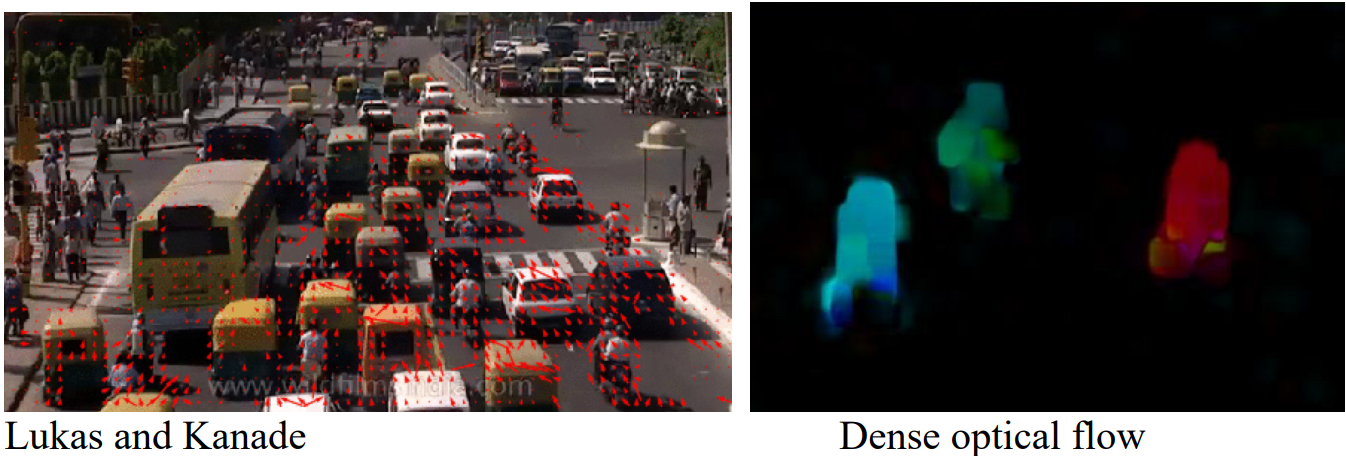
\includegraphics[width=0.7\linewidth]{_images/instructions2c}
			%\caption{}
			%\label{fig:instructions2c}
		\end{figure}
		Note that you may (or maybe not) have problems with memory (video is a sequence
		of many images), you should be able to handle that.
	\end{enumerate}


I've used my own footage (actually several videos) but they partly didn't look so good where there are a few reasons for, like the light direction. Therefore I've decided to use a Youtube video (\href{https://youtu.be/e_WBuBqS9h8}{Cars Driving By}) too. 
\begin{enumerate}[{Part} a.]
	\item \textbf{Lukas and Kanade (Sparse) Optical Flow Estimation}\\
	\textbf{Changes to the code}
	\begin{enumerate}[1.]
		\item Shi-Tomasi\\
		The Shi-Tomasi LK-OF code has been provided by OpenCV above. Shi-Tomasi is a corner detection algorithm which seeks to find good corners for stable tracking.
		
		\item SIFT\\
		In contrast to Shi-Tomasi, SIFT does not seek corners but instead robust, scale invariant features which often lie on edges or corners because the entropy there is higher than for example a mostly plain (homogeneous) plane.
		\\
		The changes to the given code can be kept to a minimum.
		\begin{lstlisting}[language=python]
sift = cv.SIFT_create(nfeatures=feature_params['maxCorners'])
kp = sift.detect(old_gray, None)
kp_pos = [[np.float32(keypt.pt)] for keypt in kp]
p0 = np.array(kp_pos)
\end{lstlisting}
	Is used instead of
	\begin{lstlisting}[language=python]
p0 = cv.goodFeaturesToTrack(old_gray, mask = None, **feature_params)
\end{lstlisting}
The number of features is limited to the same as the Shi-Tomasi detector. Otherwise SIFT would detect many more keypoints.
	\end{enumerate}

\textbf{Output of several videos}

\begin{figure}[H]
	\centering
	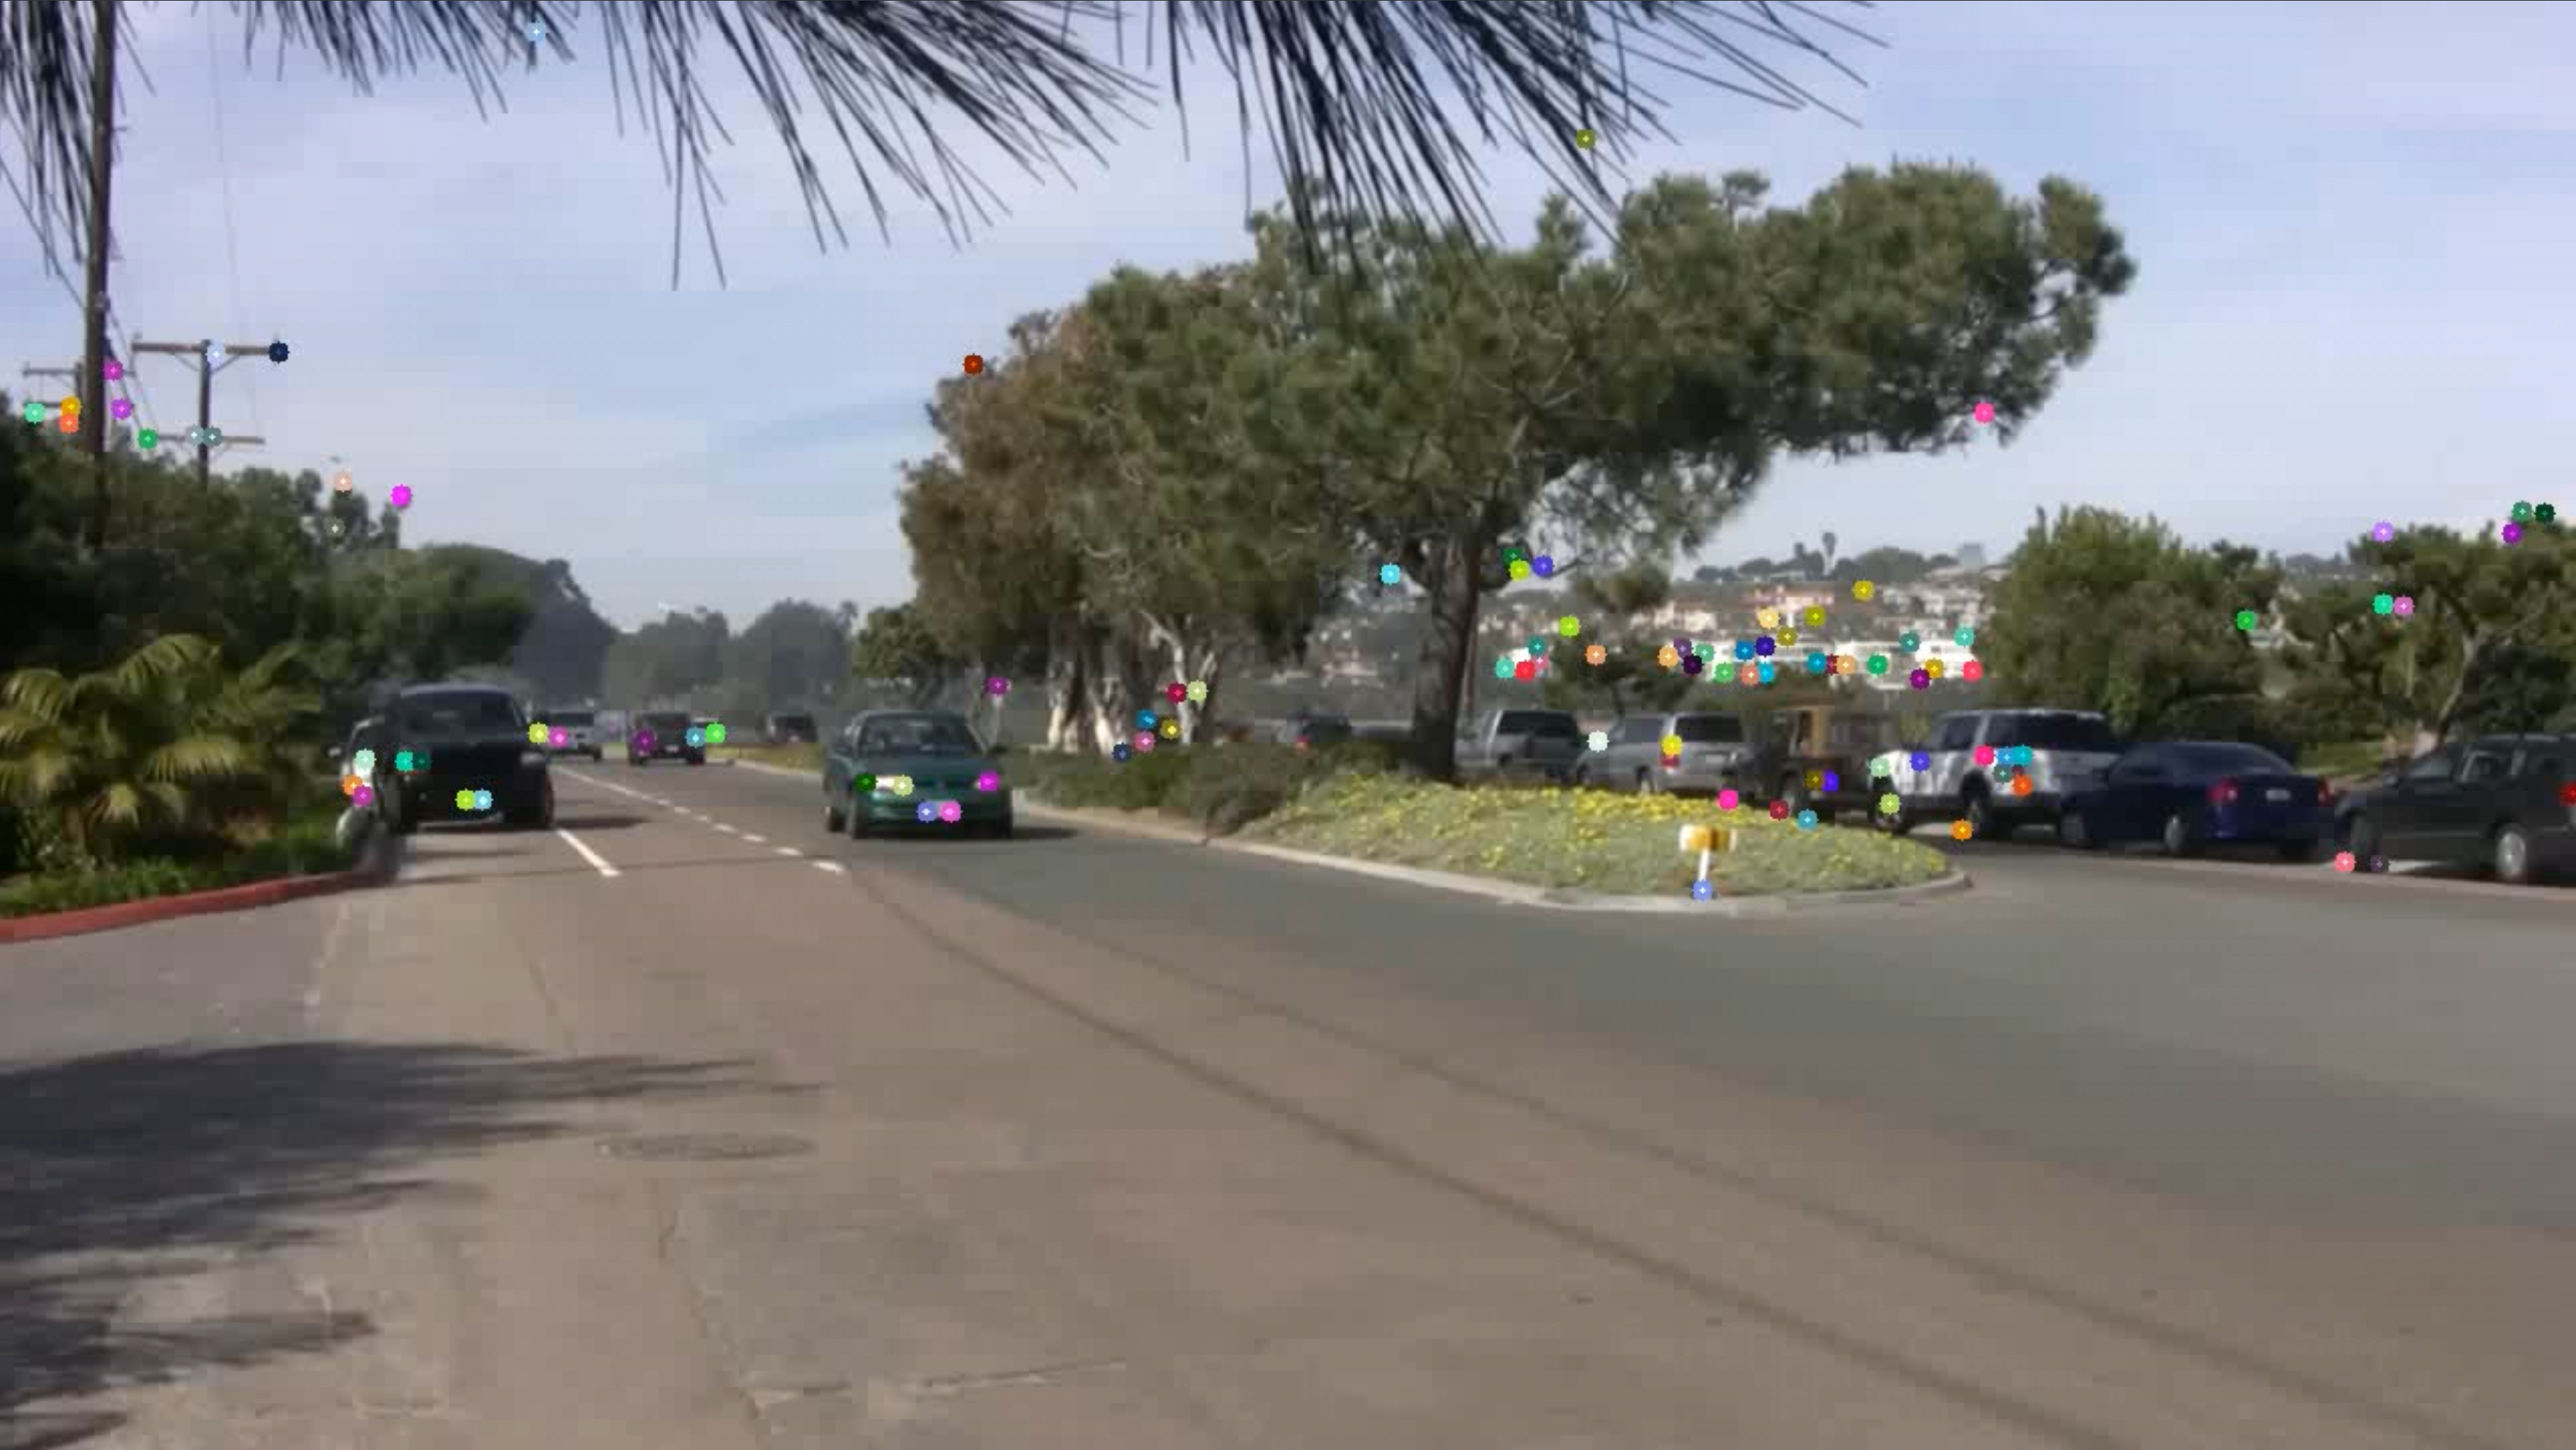
\includegraphics[width=0.5\linewidth]{_images/shi-tomasi_cars1}
	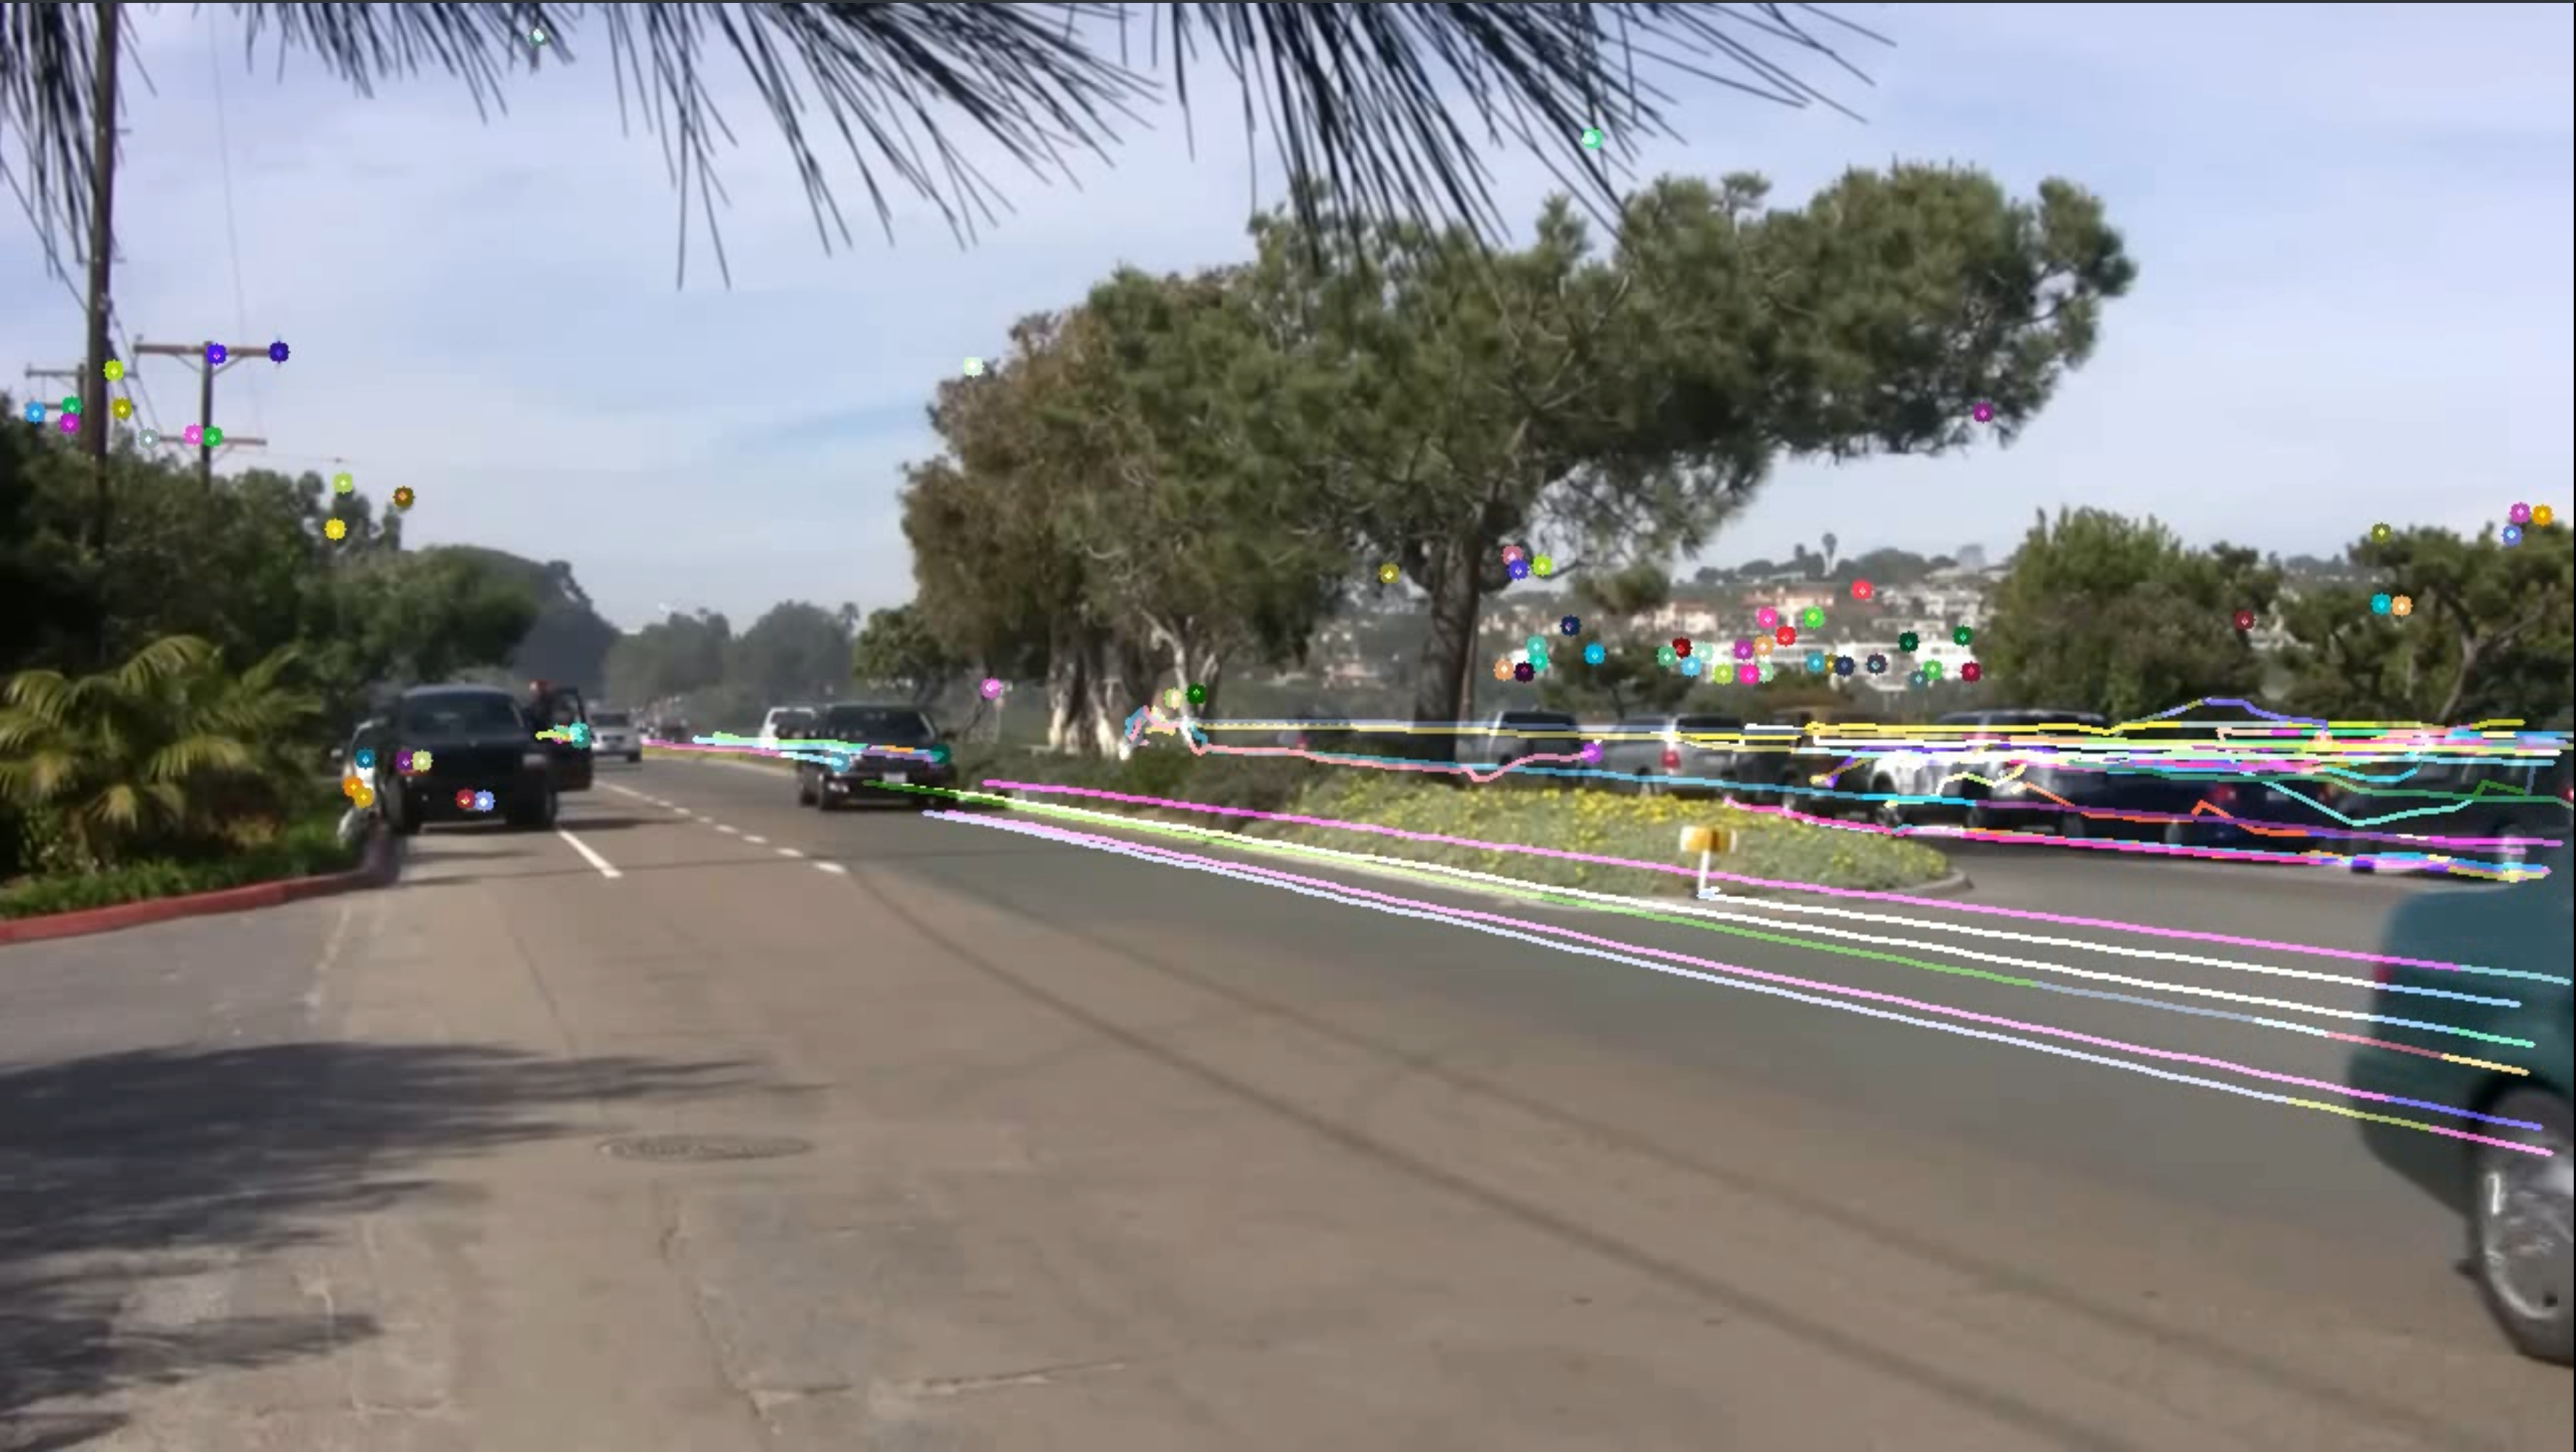
\includegraphics[width=0.5\linewidth]{_images/shi-tomasi_cars2}
	\caption{Lukas and Kanade Optical Flow using Shi-Tomasi Corner Detector. }
	\label{fig:shi-tomasicars}
\end{figure}
\begin{figure}[H]
	\centering
	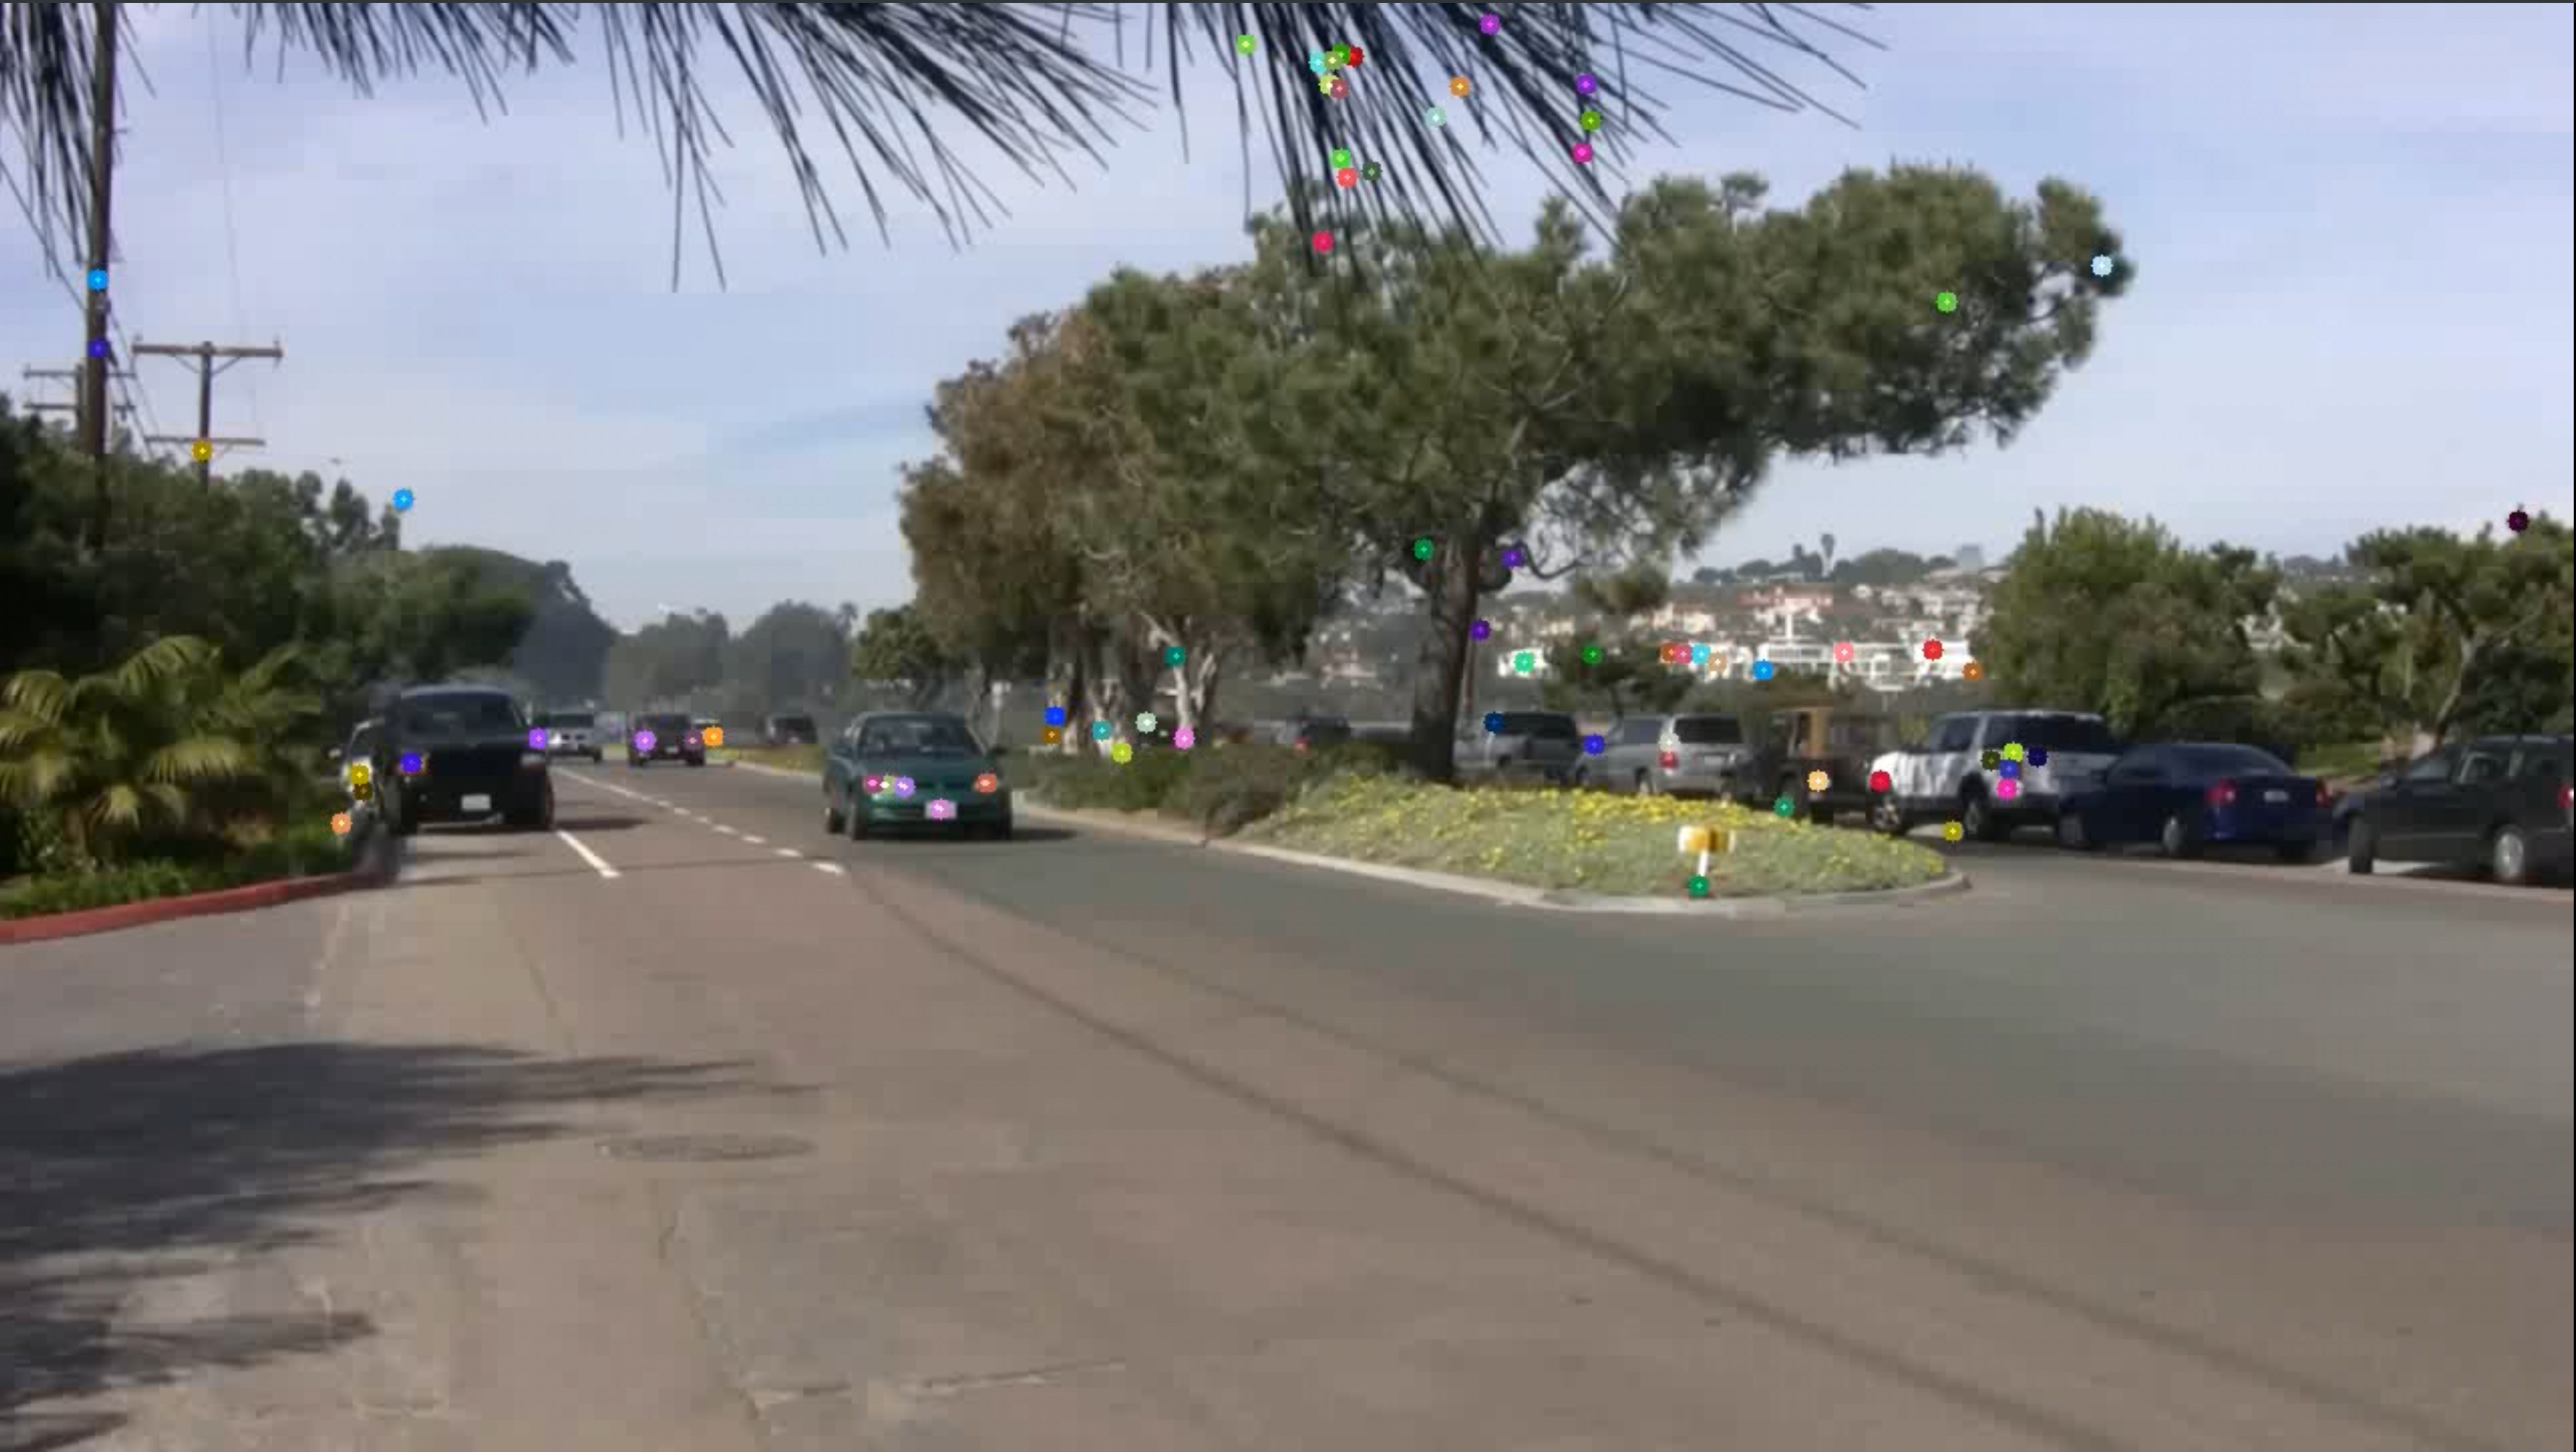
\includegraphics[width=0.5\linewidth]{_images/sift_cars1}
	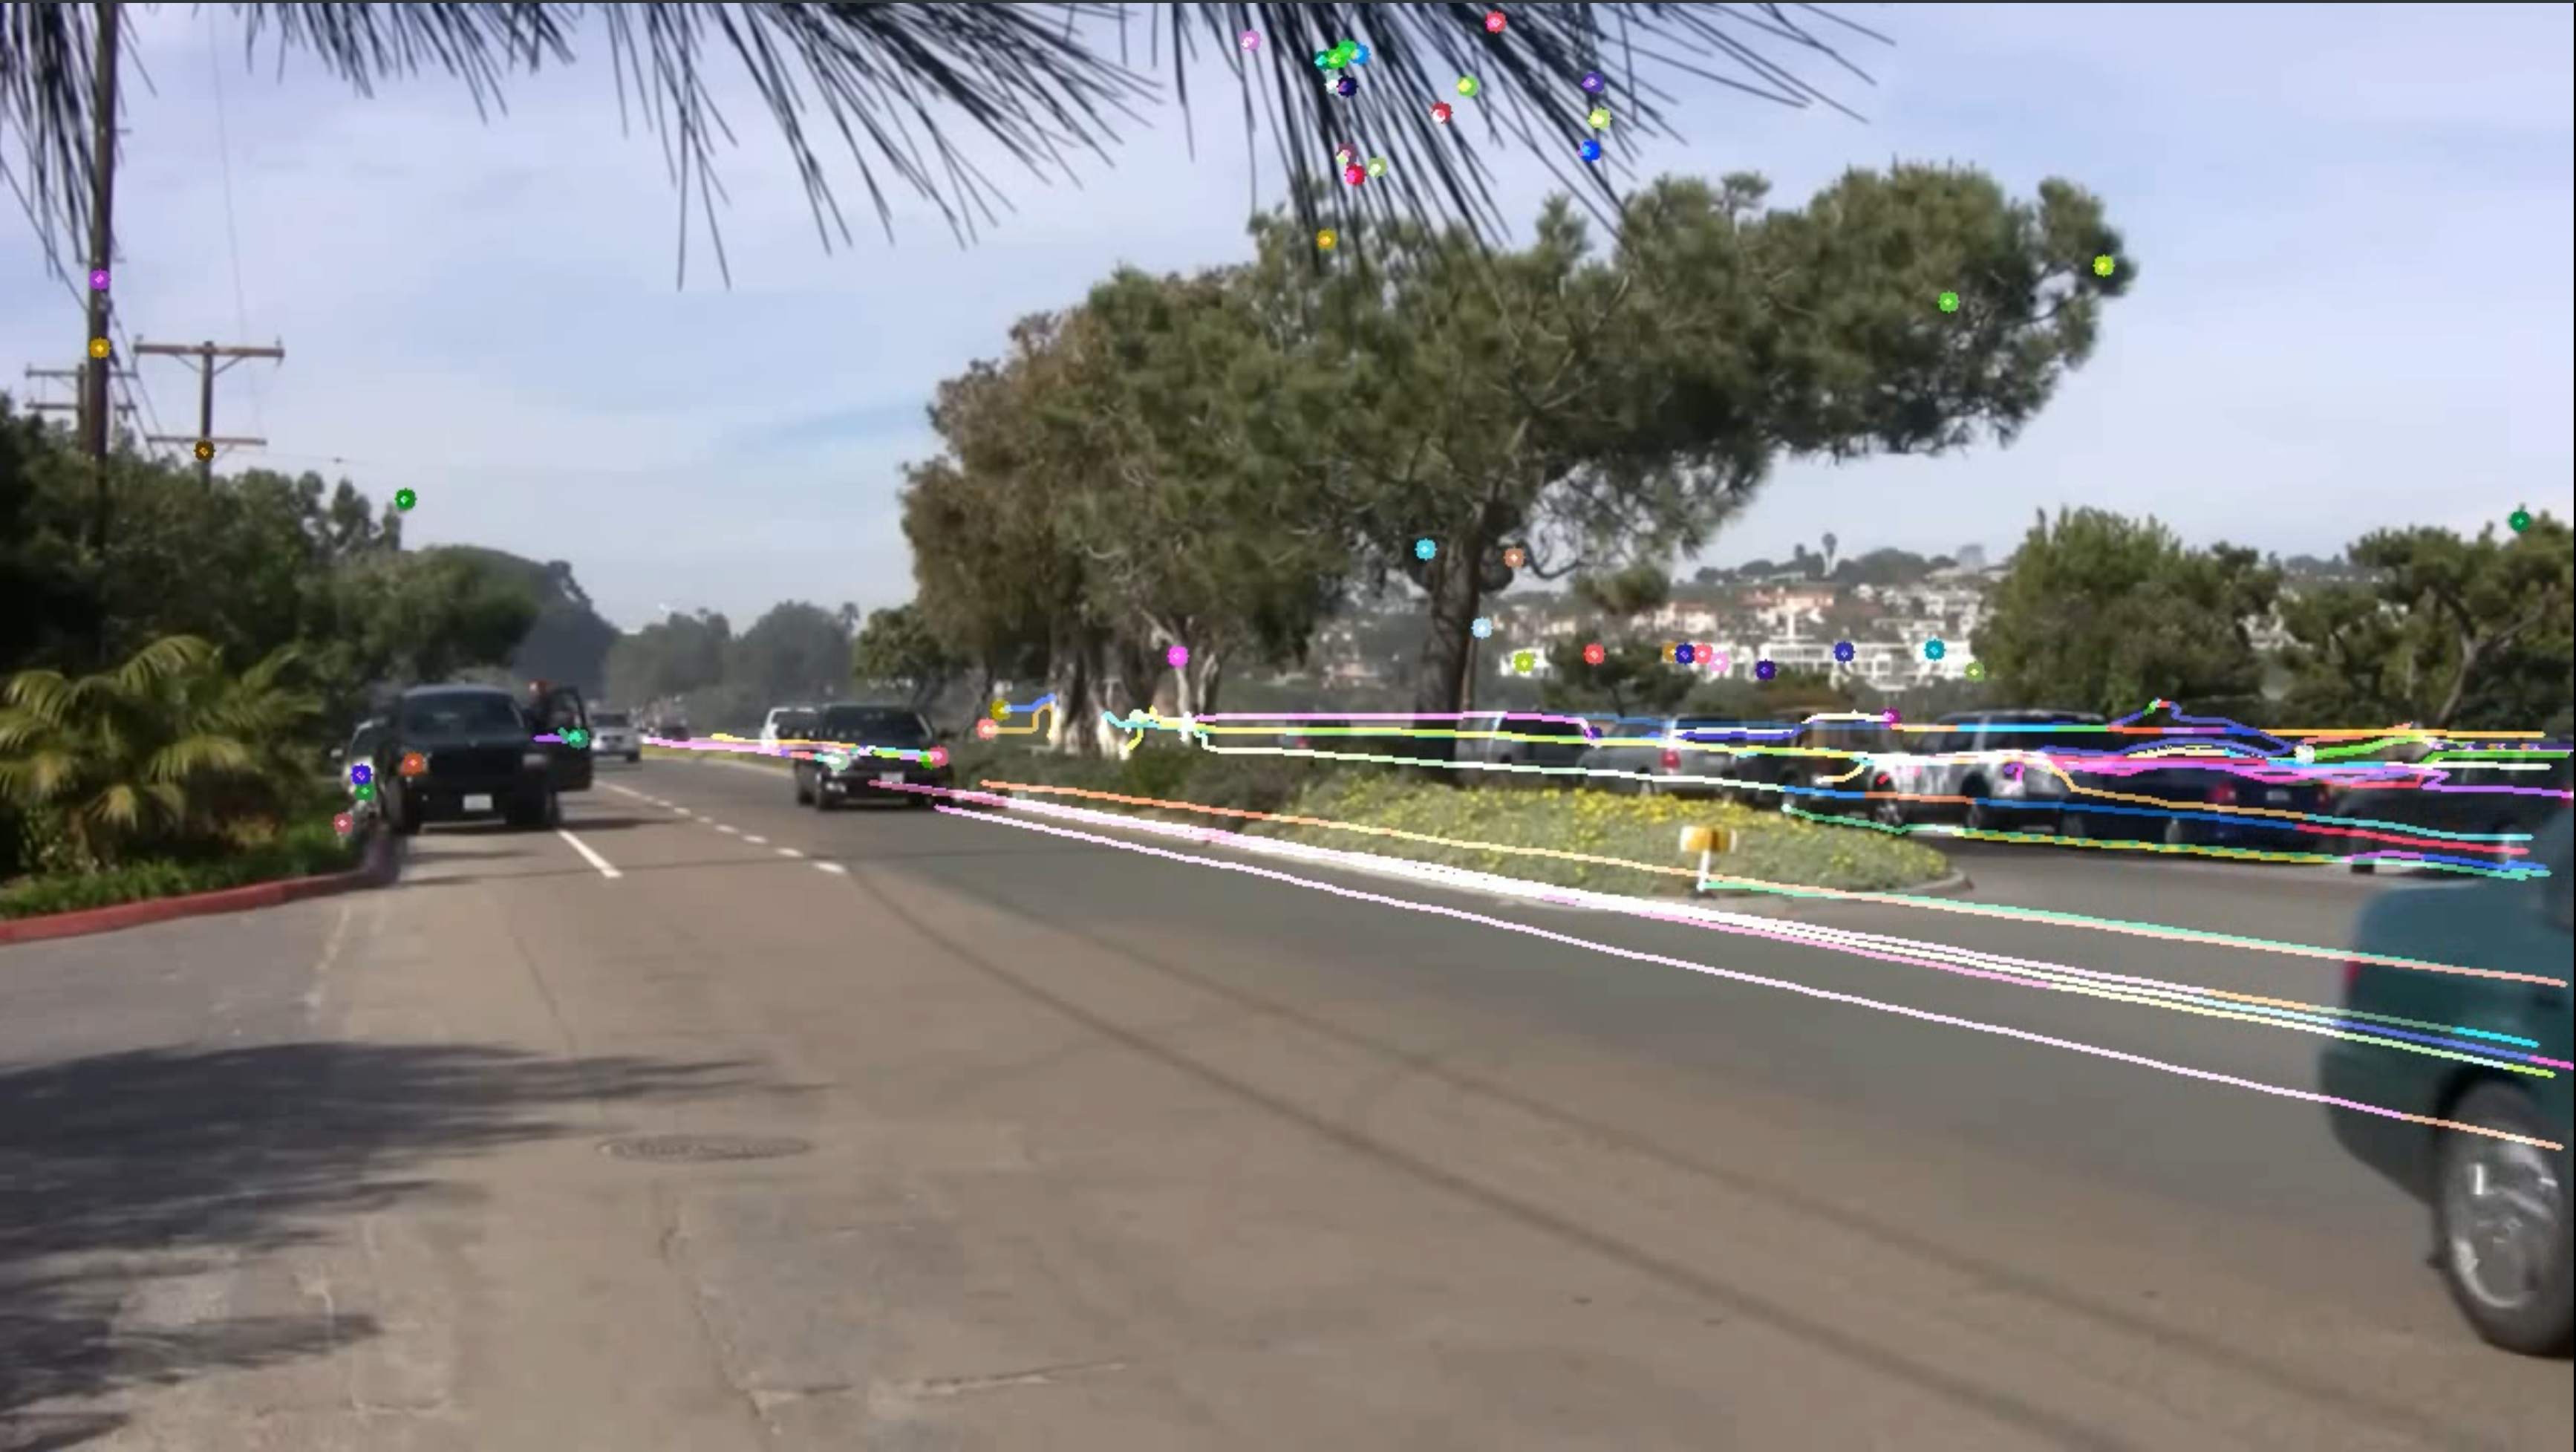
\includegraphics[width=0.5\linewidth]{_images/sift_cars2}
	\caption{Lukas and Kanade Optical Flow using SIFT. }
	\label{fig:siftcars}
\end{figure}
\begin{figure}[H]
	\centering
	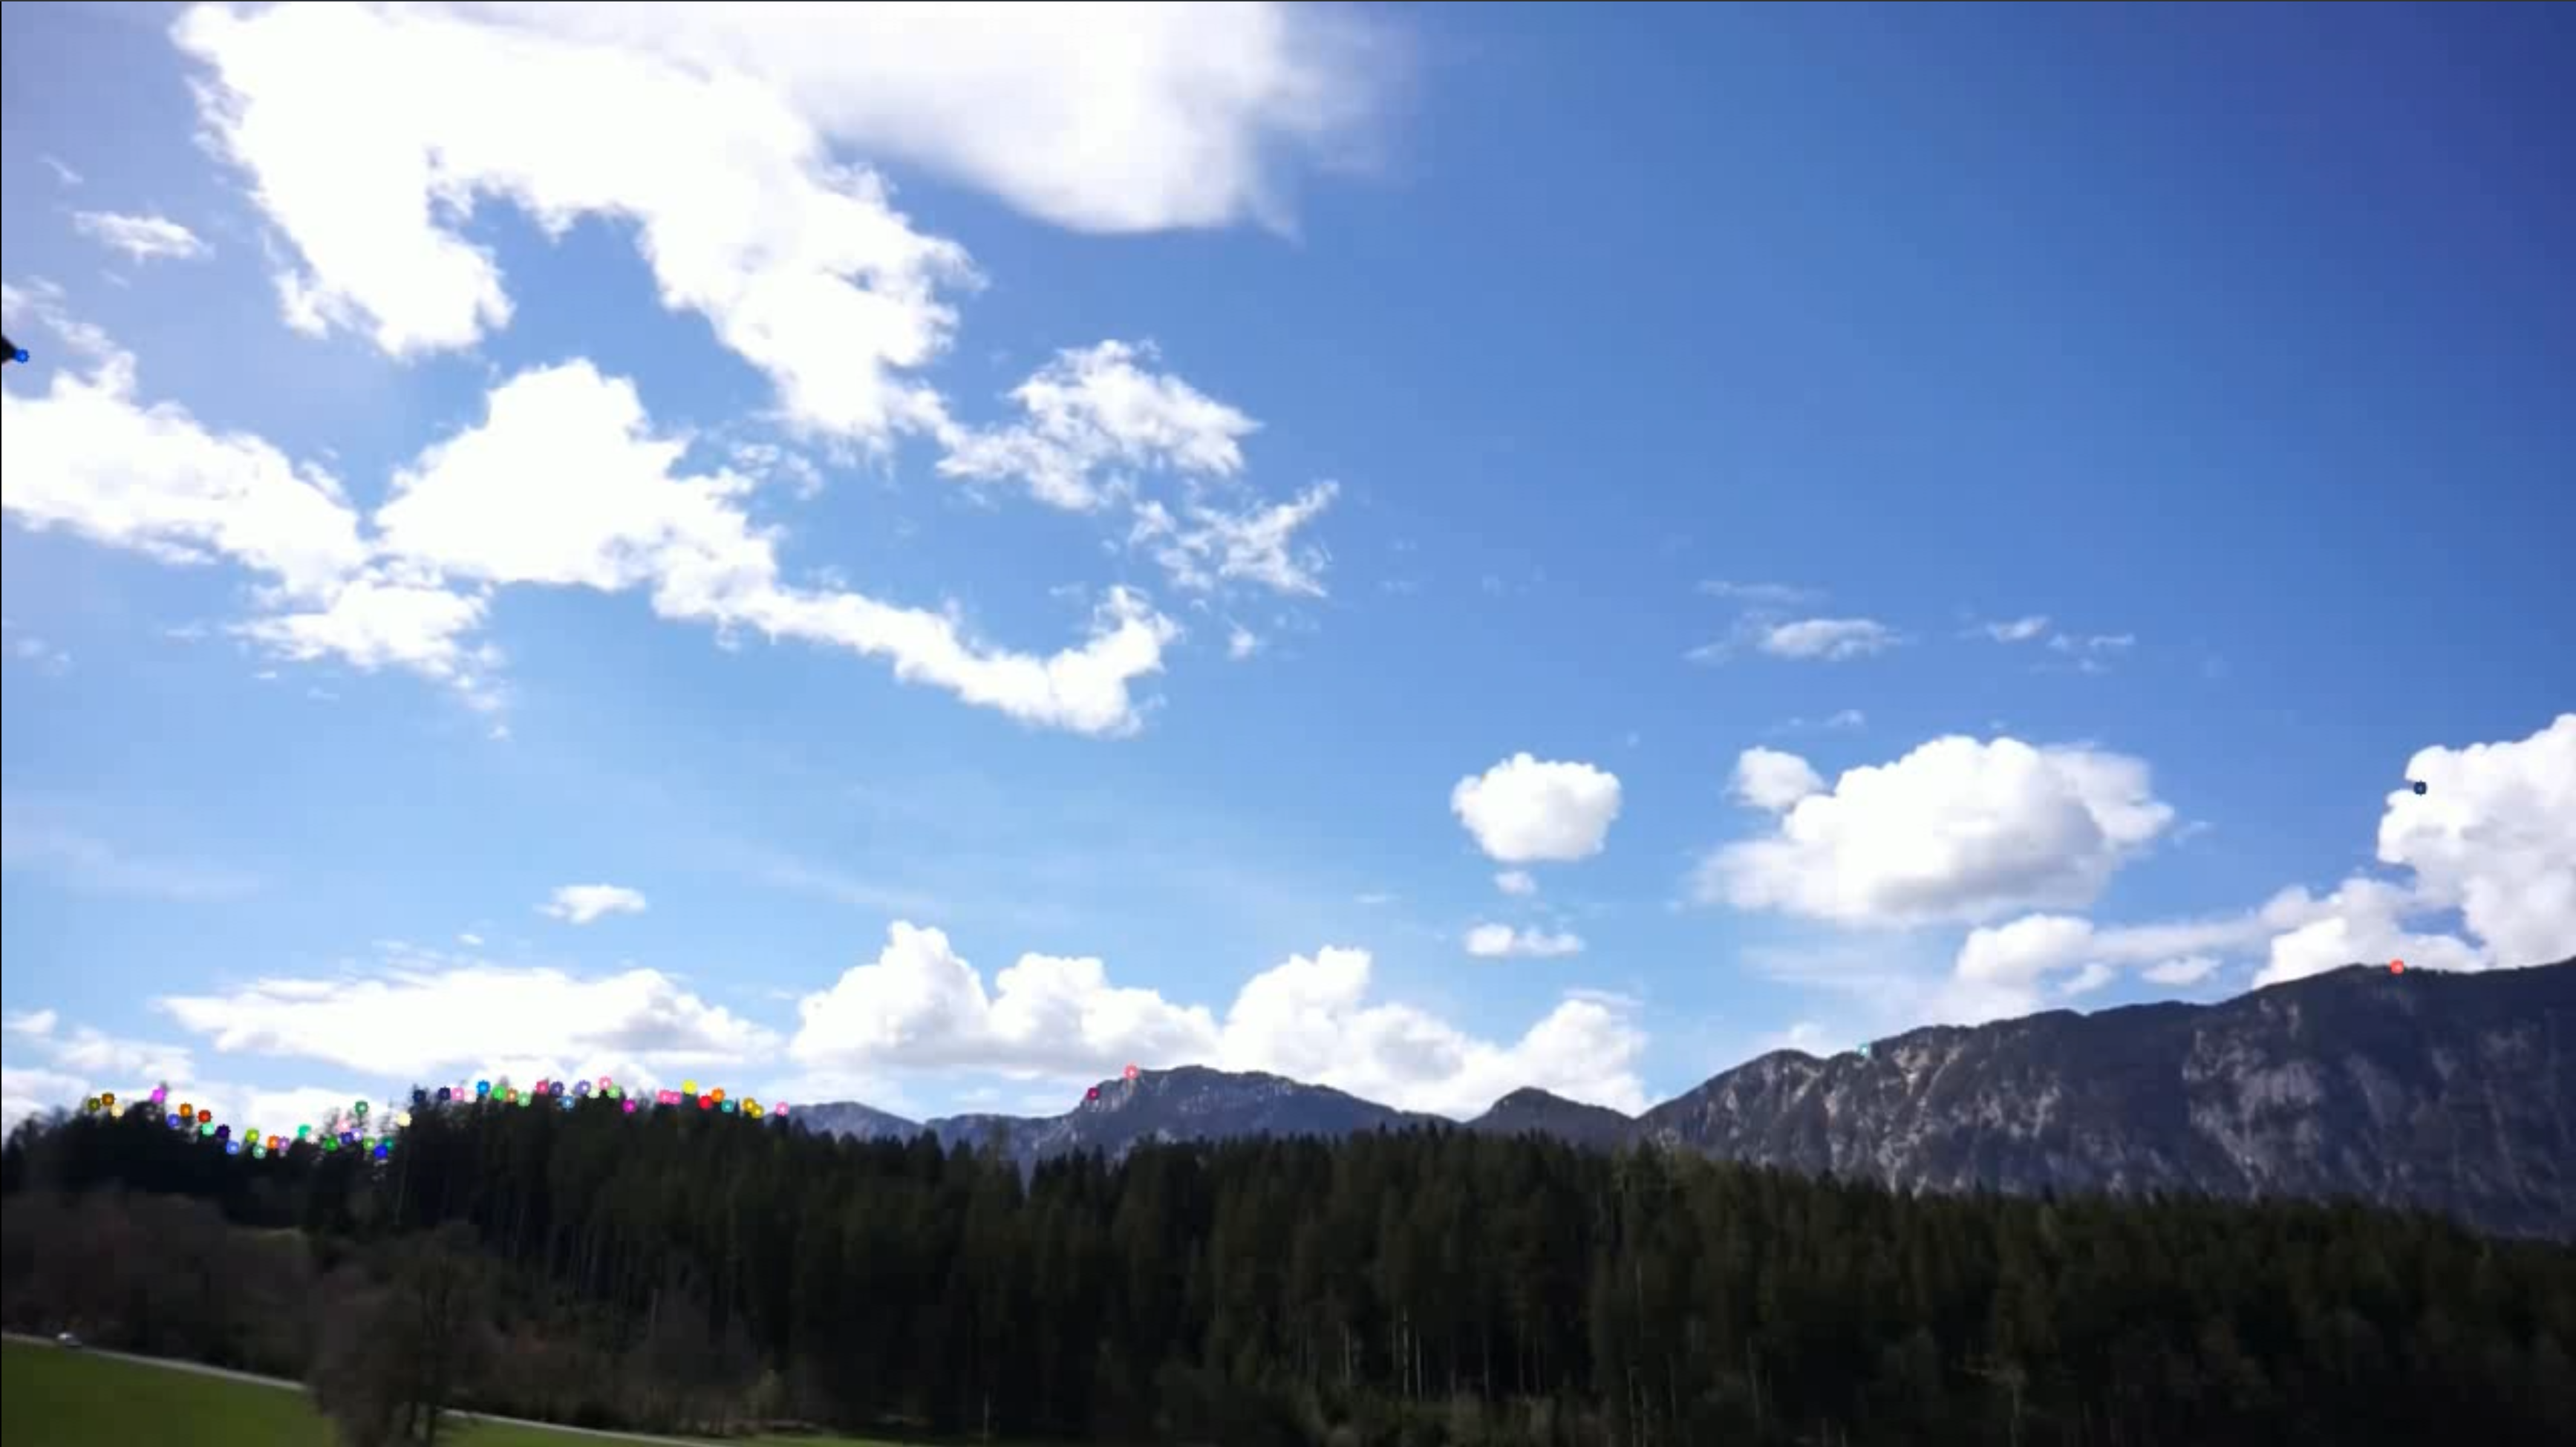
\includegraphics[width=0.9\linewidth]{_images/shi-tomasi_sky1}
	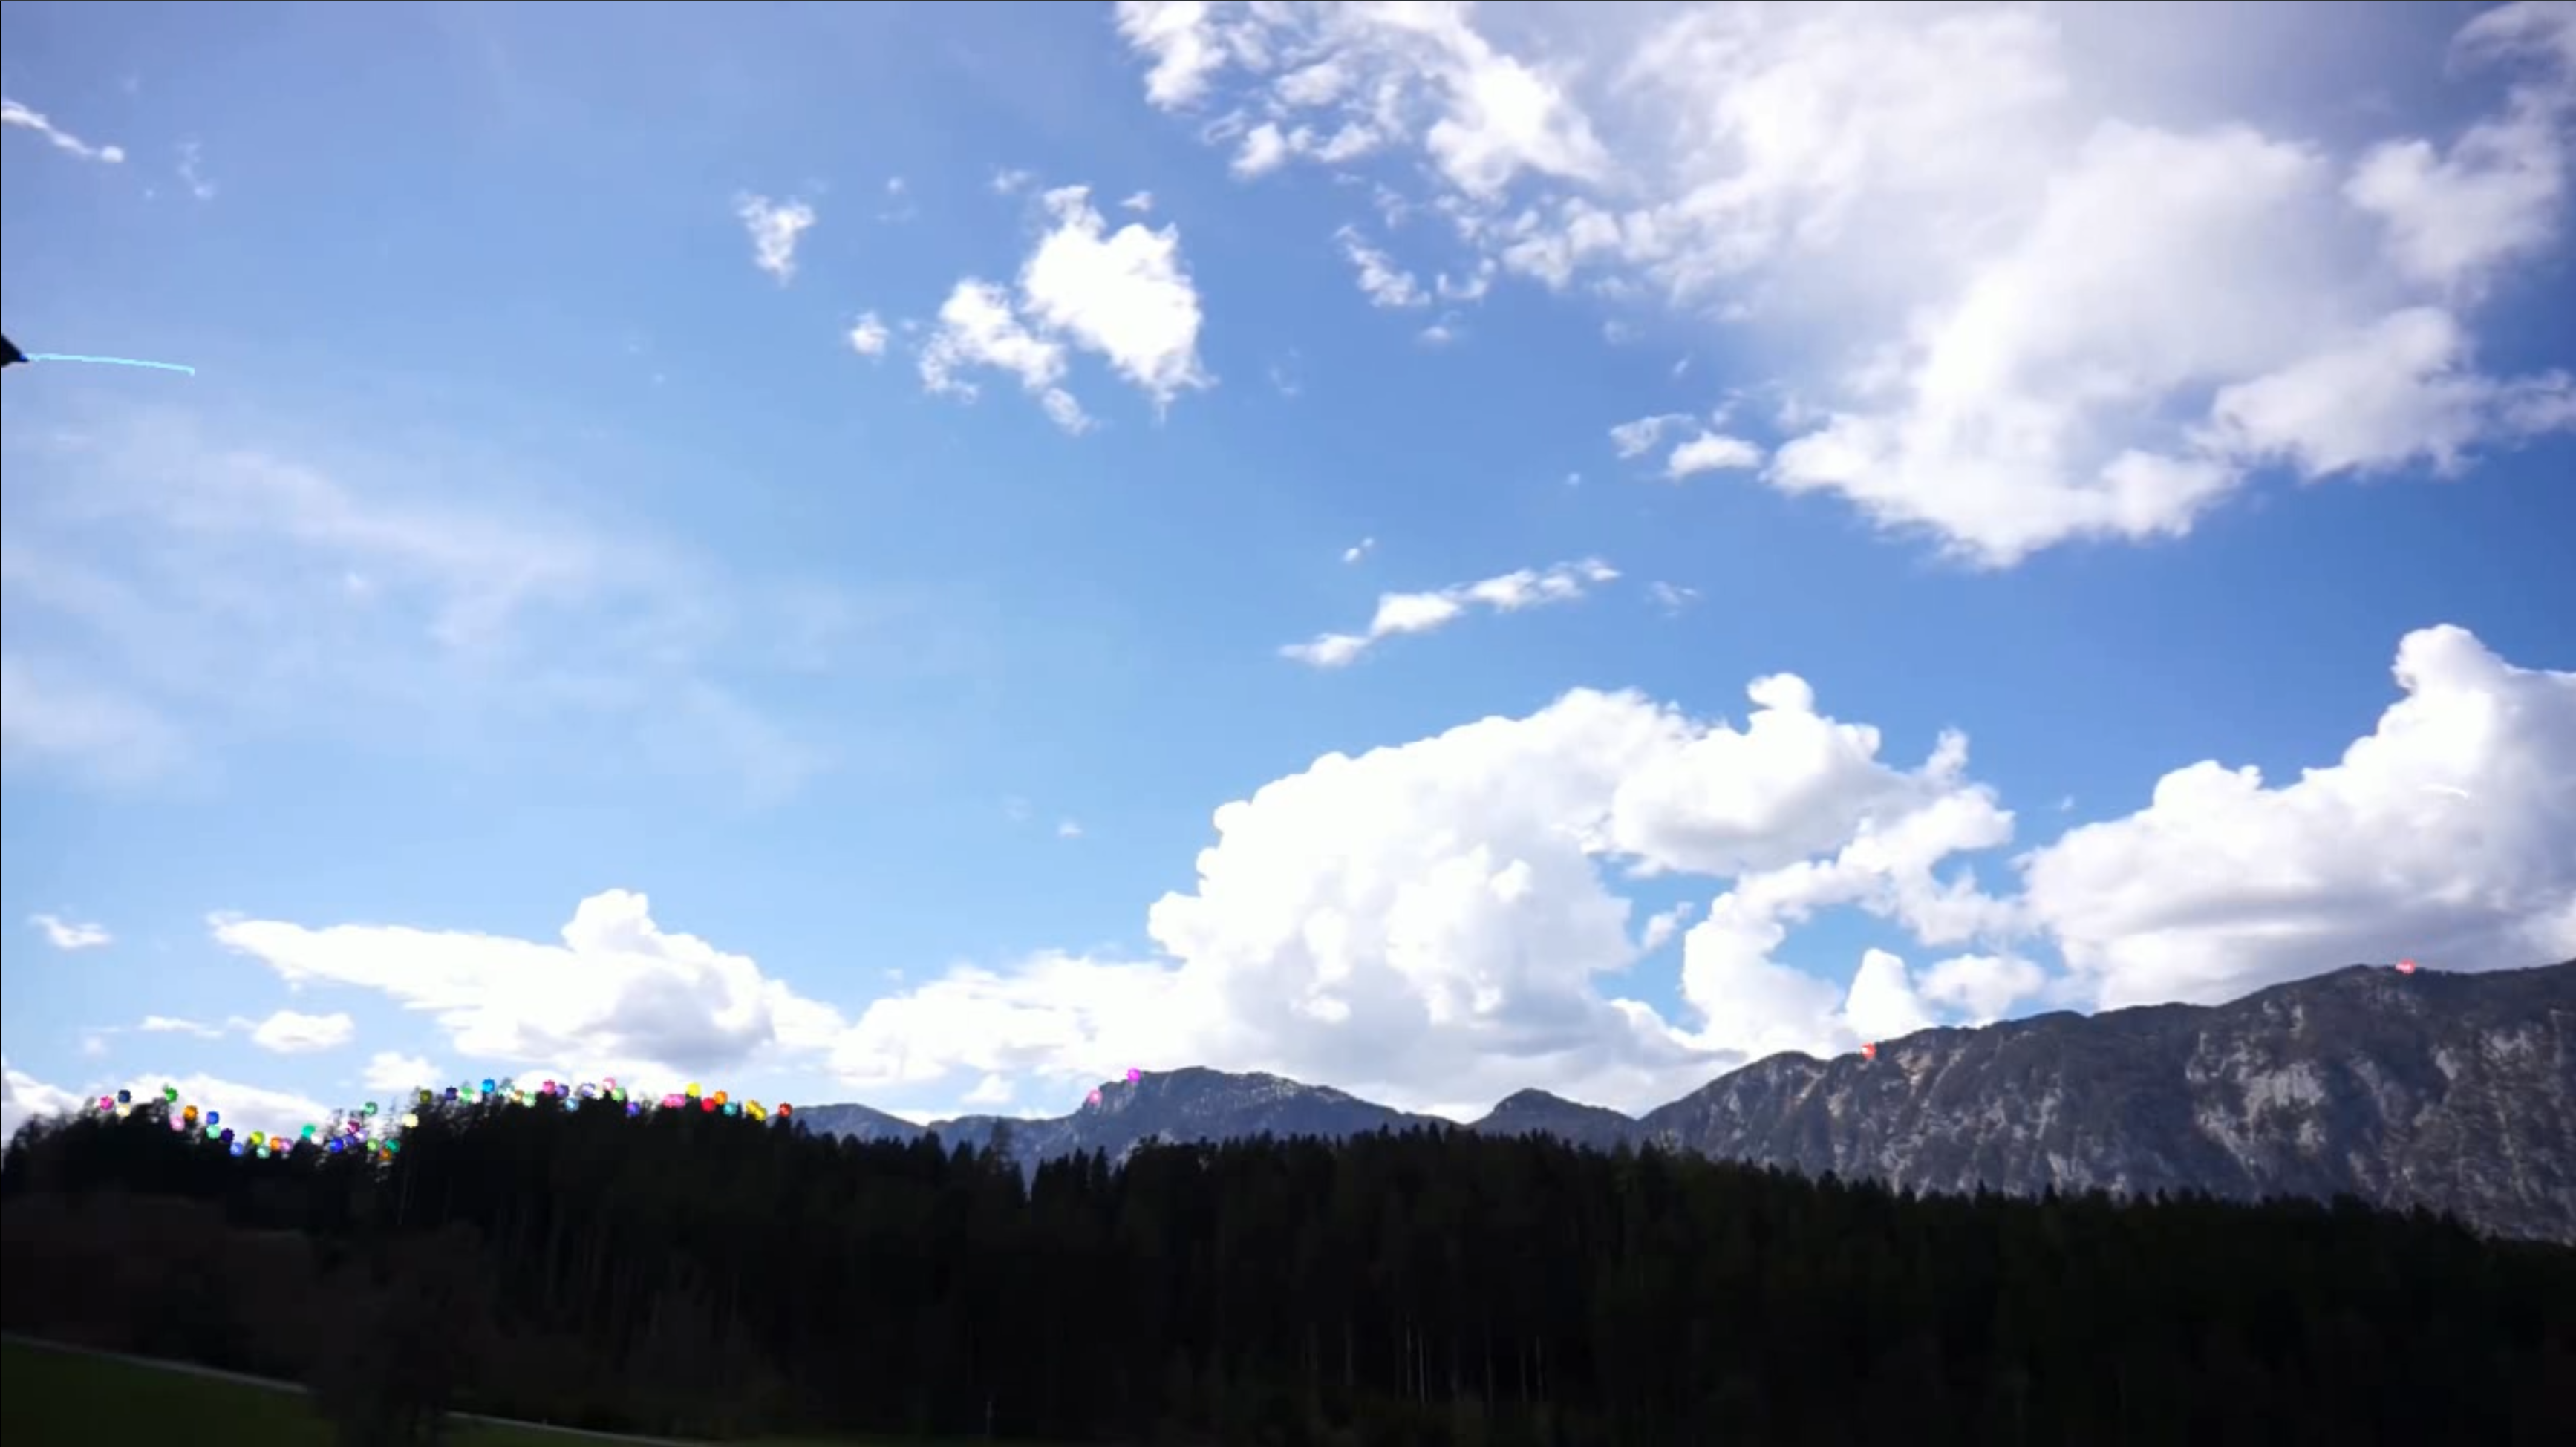
\includegraphics[width=0.9\linewidth]{_images/shi-tomasi_sky2}
	\caption{Lukas and Kanade Optical Flow using Shi-Tomasi Corner Detector. }
	\label{fig:shi-tomasisky}
\end{figure}
\begin{figure}[H]
	\centering
	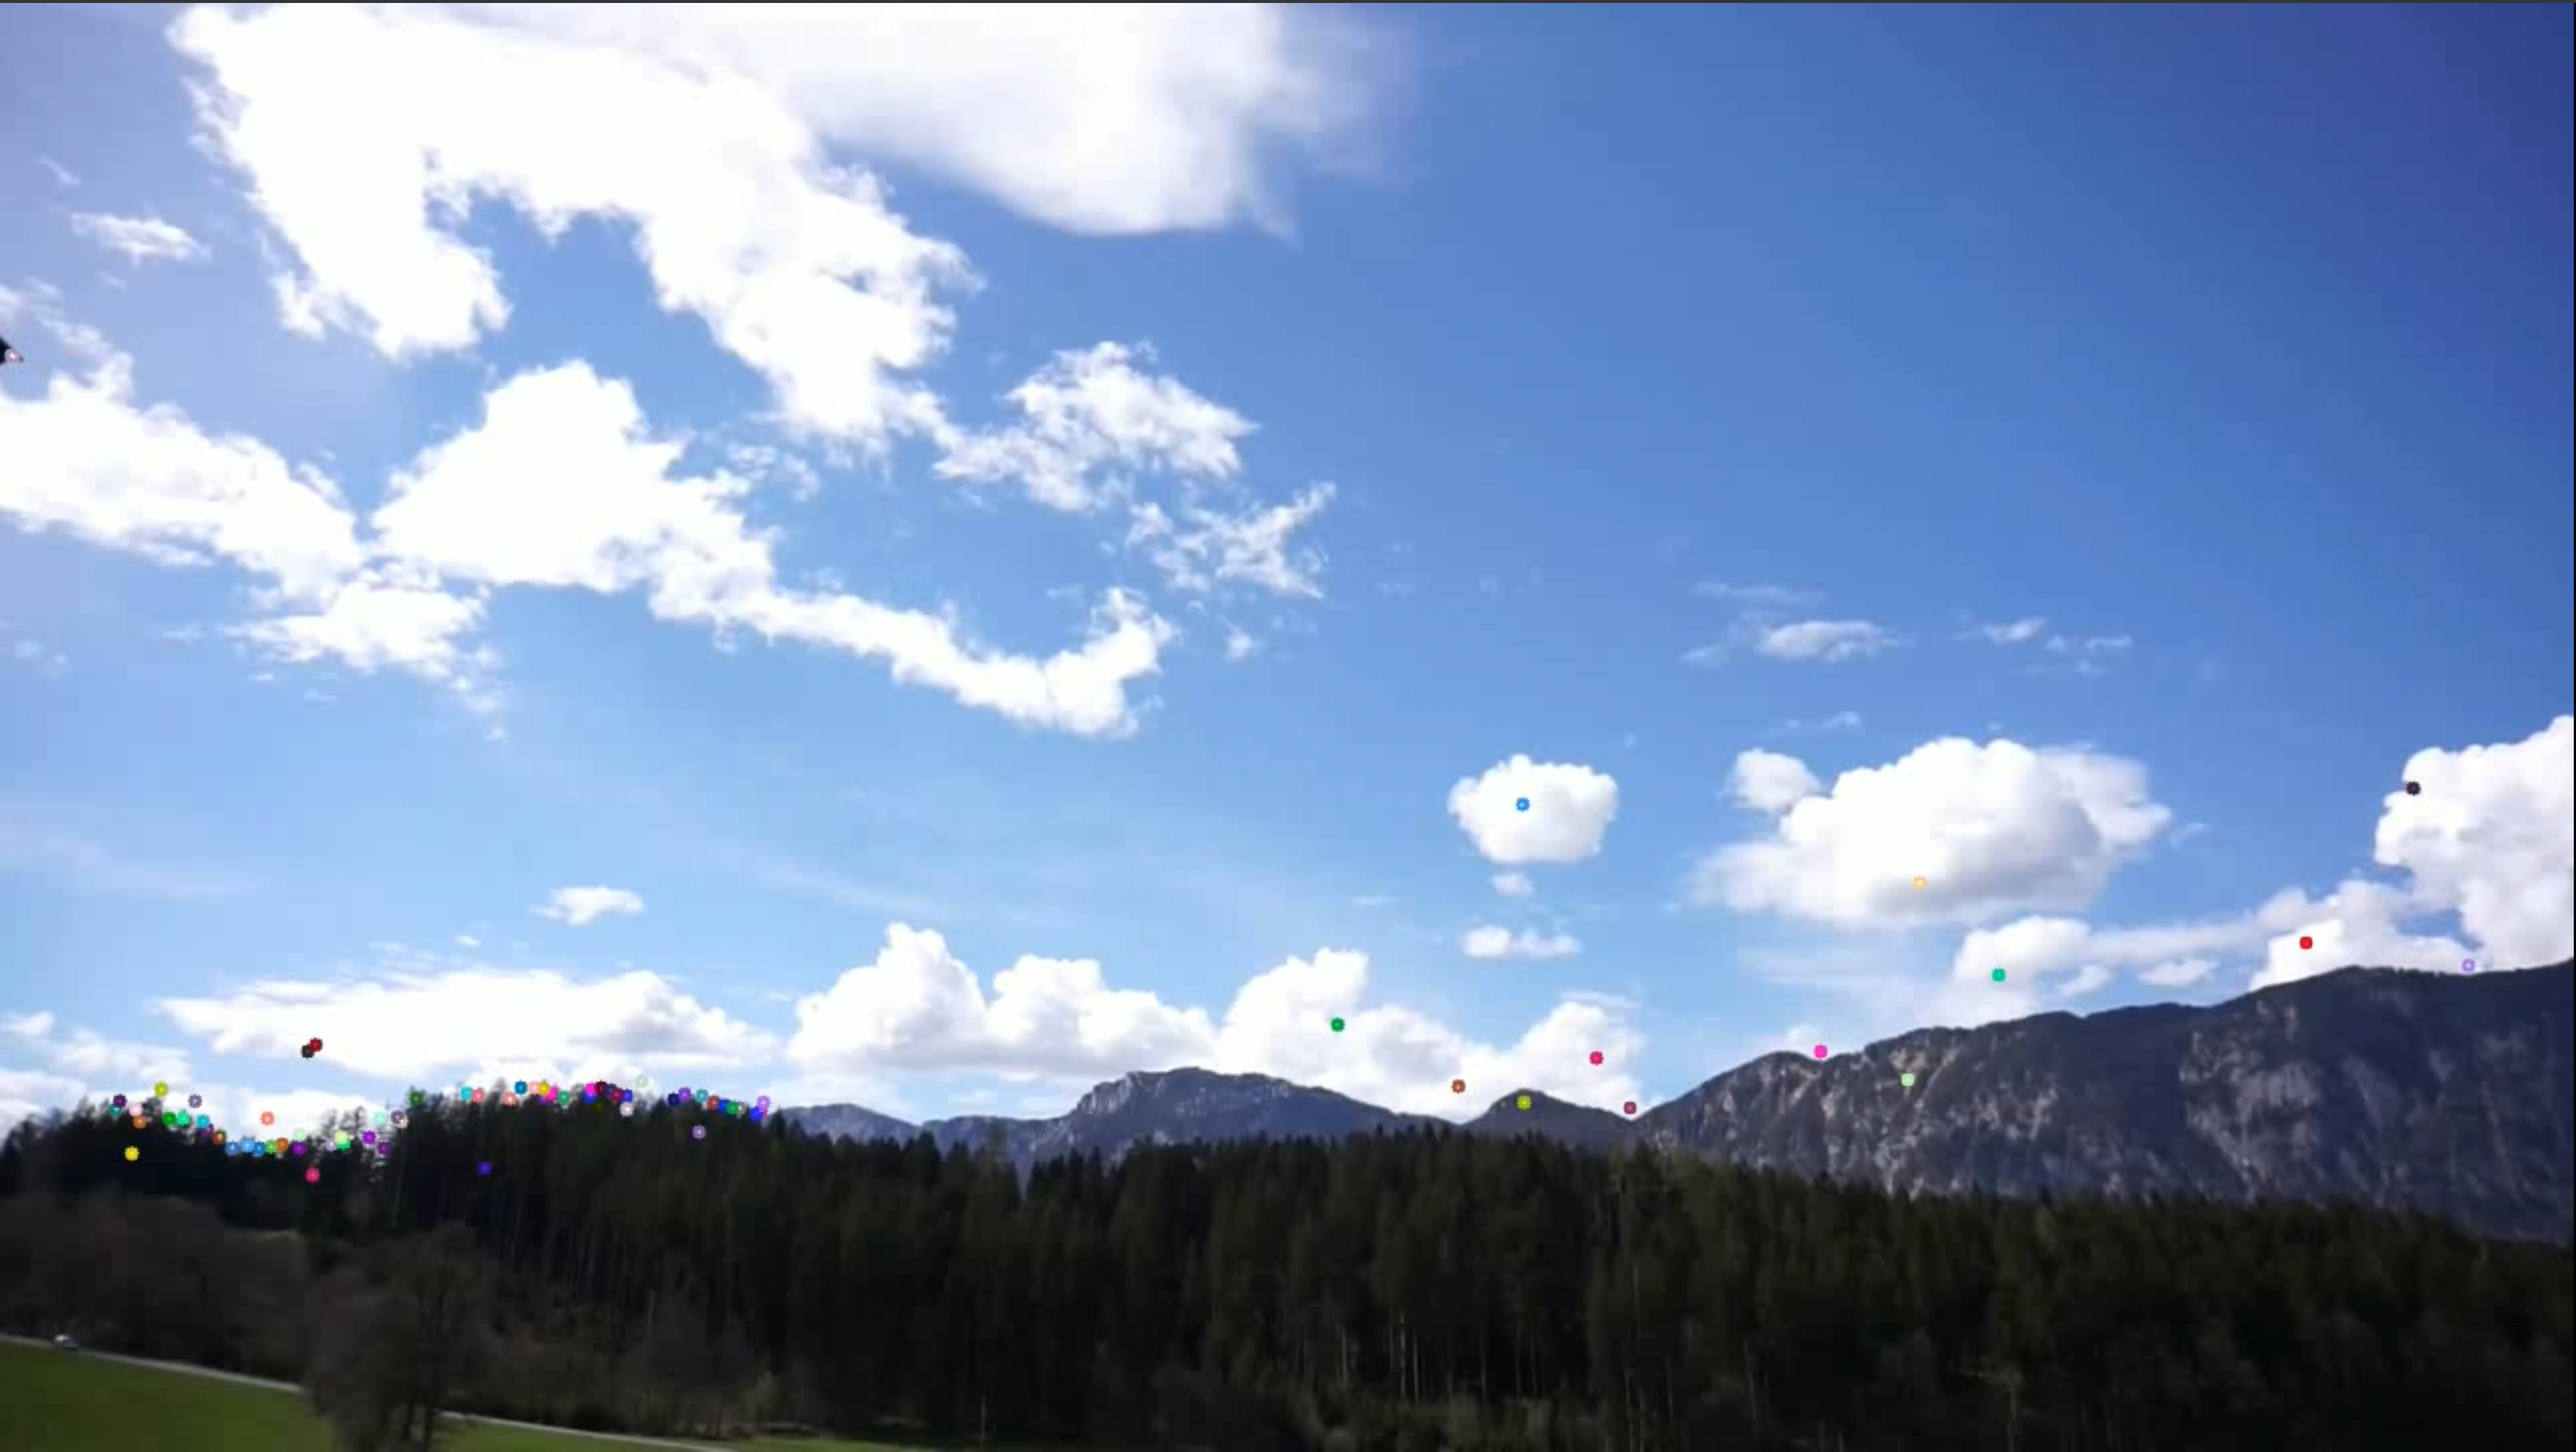
\includegraphics[width=0.9\linewidth]{_images/sift_sky1}
	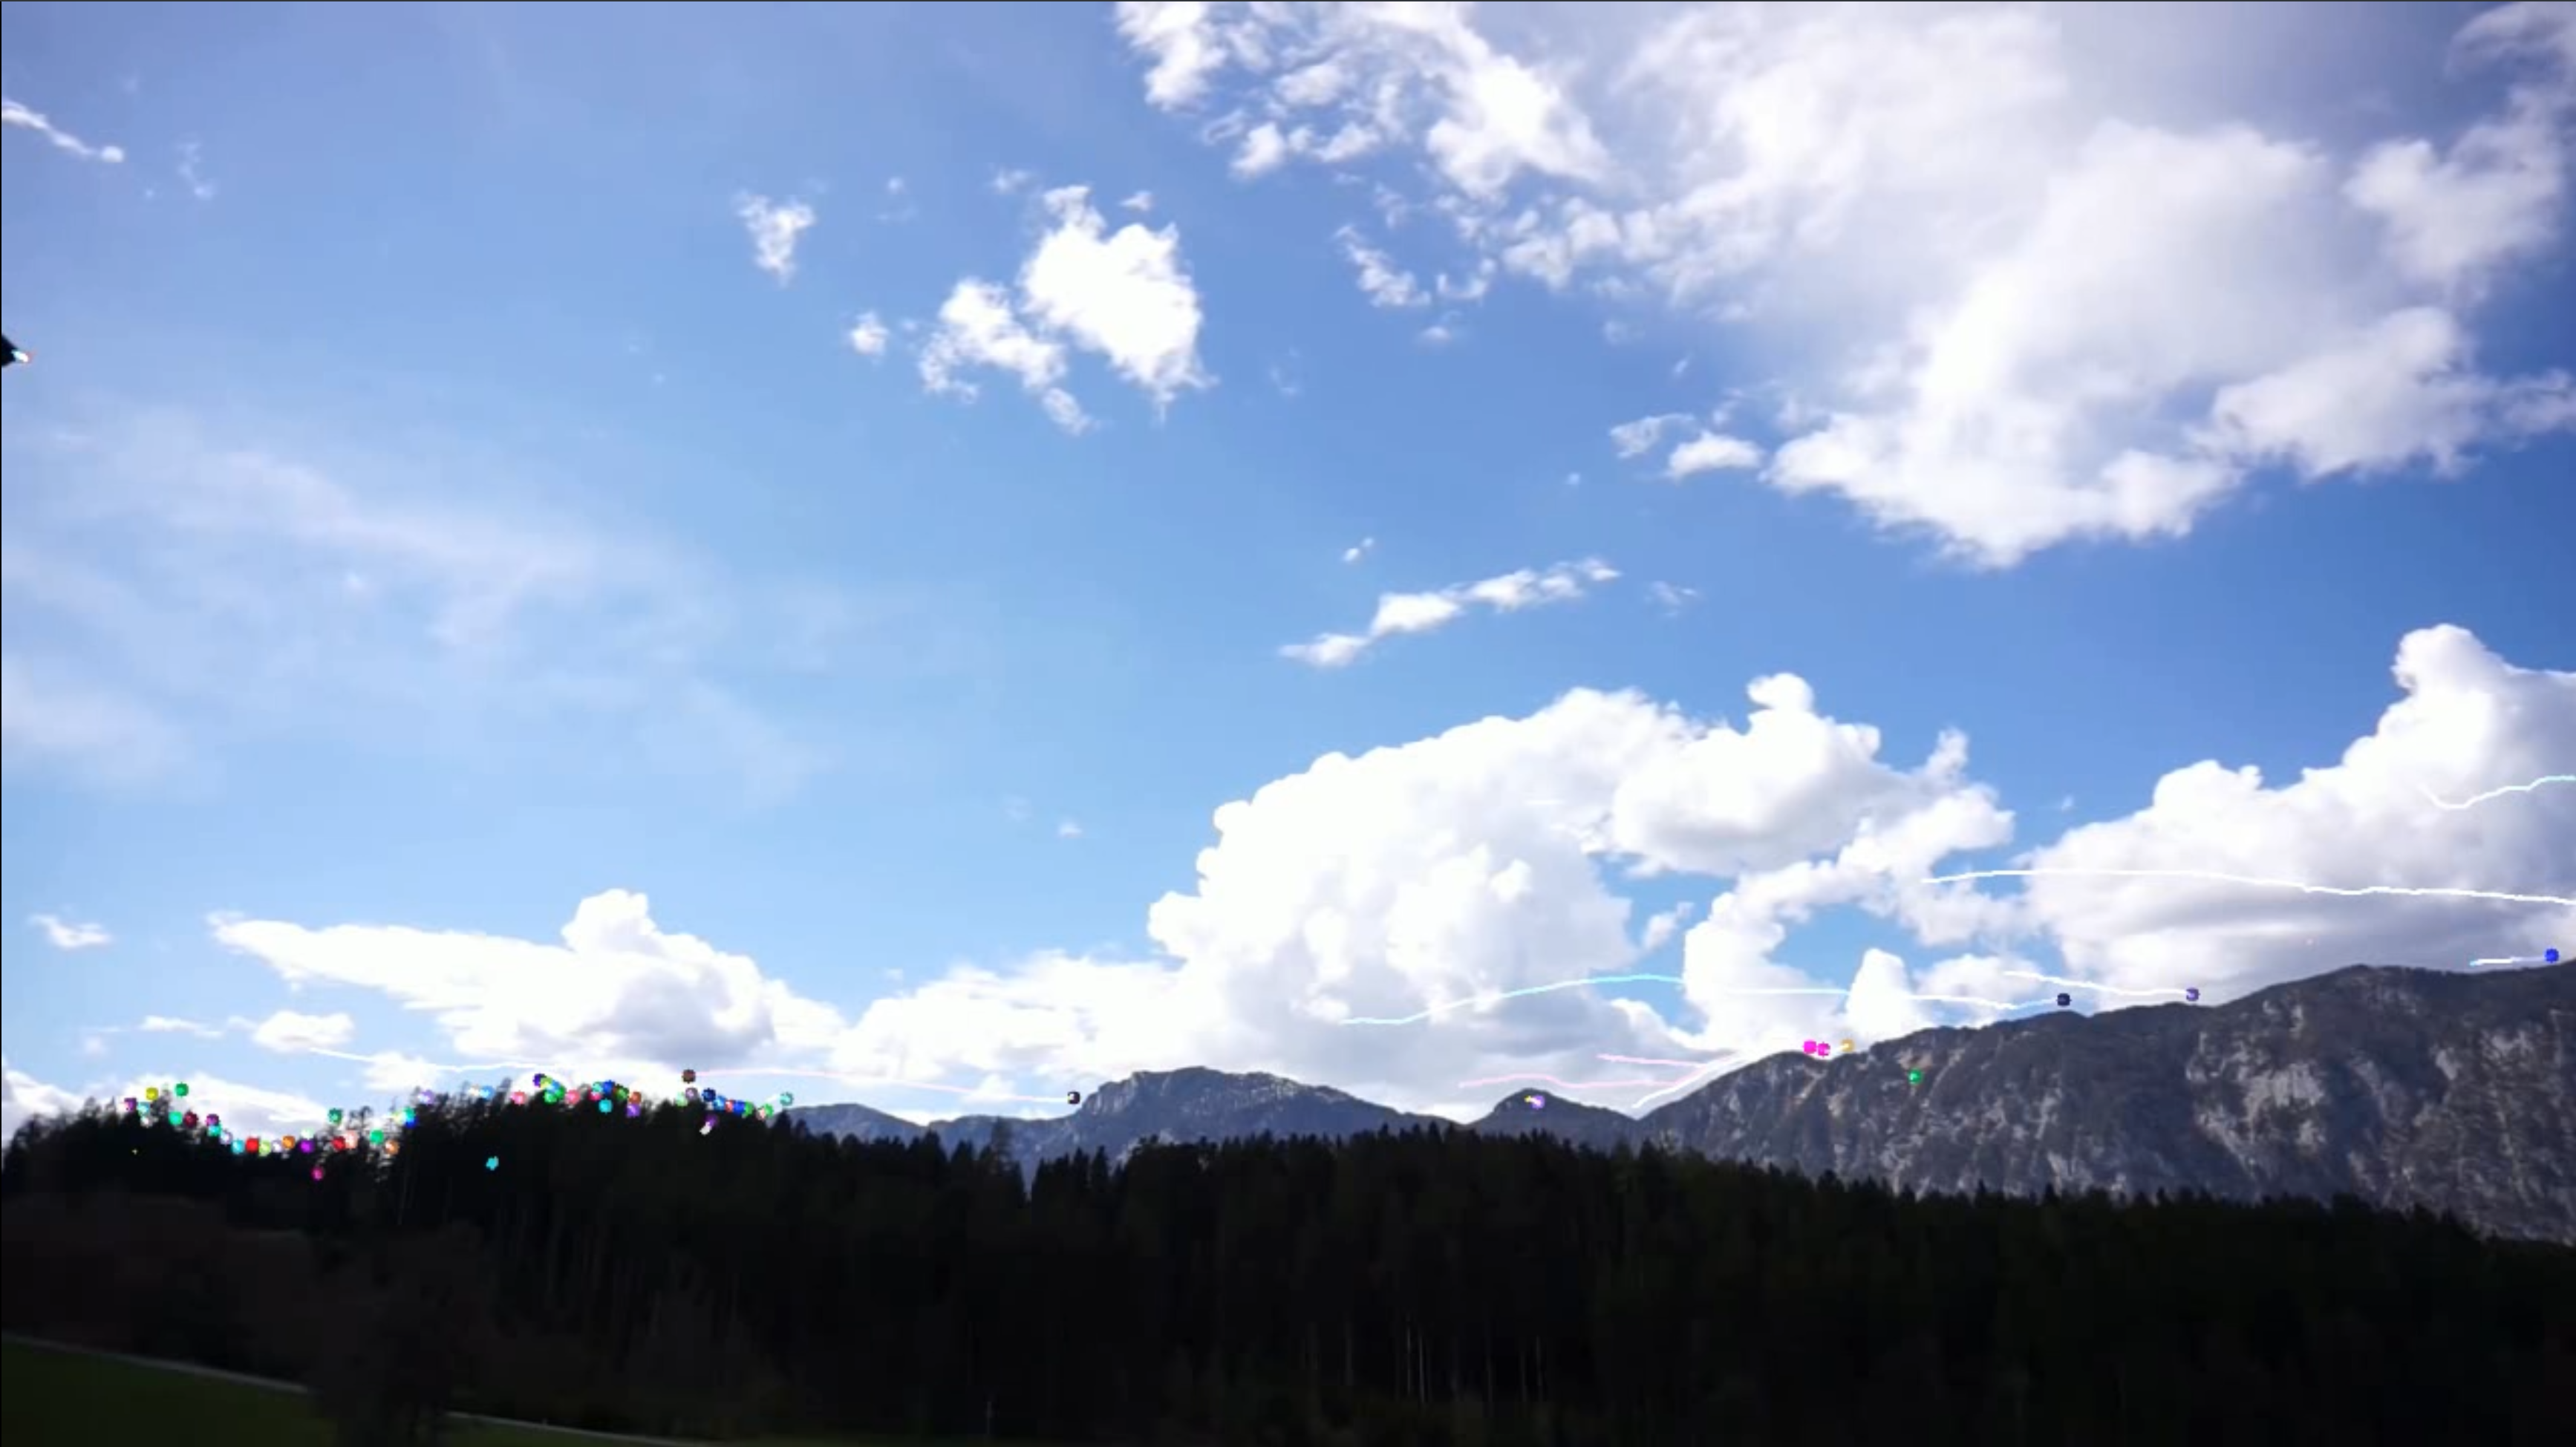
\includegraphics[width=0.9\linewidth]{_images/sift_sky2}
	\caption{Lukas and Kanade Optical Flow using SIFT.}
	\label{fig:siftsky}
\end{figure}


\textbf{Evaluation and discussion of the sparse OF algorithms}
Looking at the above images it is obvious that Shi-Tomasi Corner detector chooses vastly different key points than SIFT. Comparing figures \ref{fig:shi-tomasicars} and \ref{fig:siftcars}, SIFT marked the leafs of the tree in front top. Also Shi-Tomasi seems to have found some "good" corners in the houses in the far background. If we look at the output after a few seconds they look relatively similar, this is due to the cars moving through a rather large part of the image. I for myself think that both algorithms made a pretty good job with this footage.\\
Now comparing the timelapse of the clouds and some Austrian mountains there is a bigger difference. In figure \ref{fig:shi-tomasisky} there is just one marker on the clouds all other ones are mostly located on the tips of the trees a few ones on the mountains. This causes that there is almost no change to the output after a few minutes. So here almost no Optical Flow is being detected.
SIFT in figure \ref{fig:siftsky} has detected a lot more key points on the clouds which is desired in this case. This results in a much better evaluation of optical flow in the below image.
	
	\item \textbf{Dense Optical Flow}
	\begin{enumerate}[1.]
		\item Farneback\\
		The Farneback Dense Optical Flow code has been provided by OpenCV. The only code I've added was to save the video output to make it simpler to look for good images for this document.
\begin{lstlisting}[language=python]
next = cv.cvtColor(frame2, cv.COLOR_BGR2GRAY)
flow = cv.calcOpticalFlowFarneback(prvs, next, None, 0.5, 3, 15, 3, 5, 1.2, 0)
mag, ang = cv.cartToPolar(flow[..., 0], flow[..., 1])
hsv[..., 0] = ang*180/np.pi/2
hsv[..., 2] = cv.normalize(mag, None, 0, 255, cv.NORM_MINMAX)
bgr = cv.cvtColor(hsv, cv.COLOR_HSV2BGR)
\end{lstlisting}
This code is the core part of the Farneback algorithm including the color and direction encoding using HSV colorspace. The parameters that were given besides the images are for the pyramid scaling, number of levels, window size, iterations, dimension for the polynomial expansion and a value for the standard deviation of the polynomial.
		
		\begin{figure}[H]
			\centering
			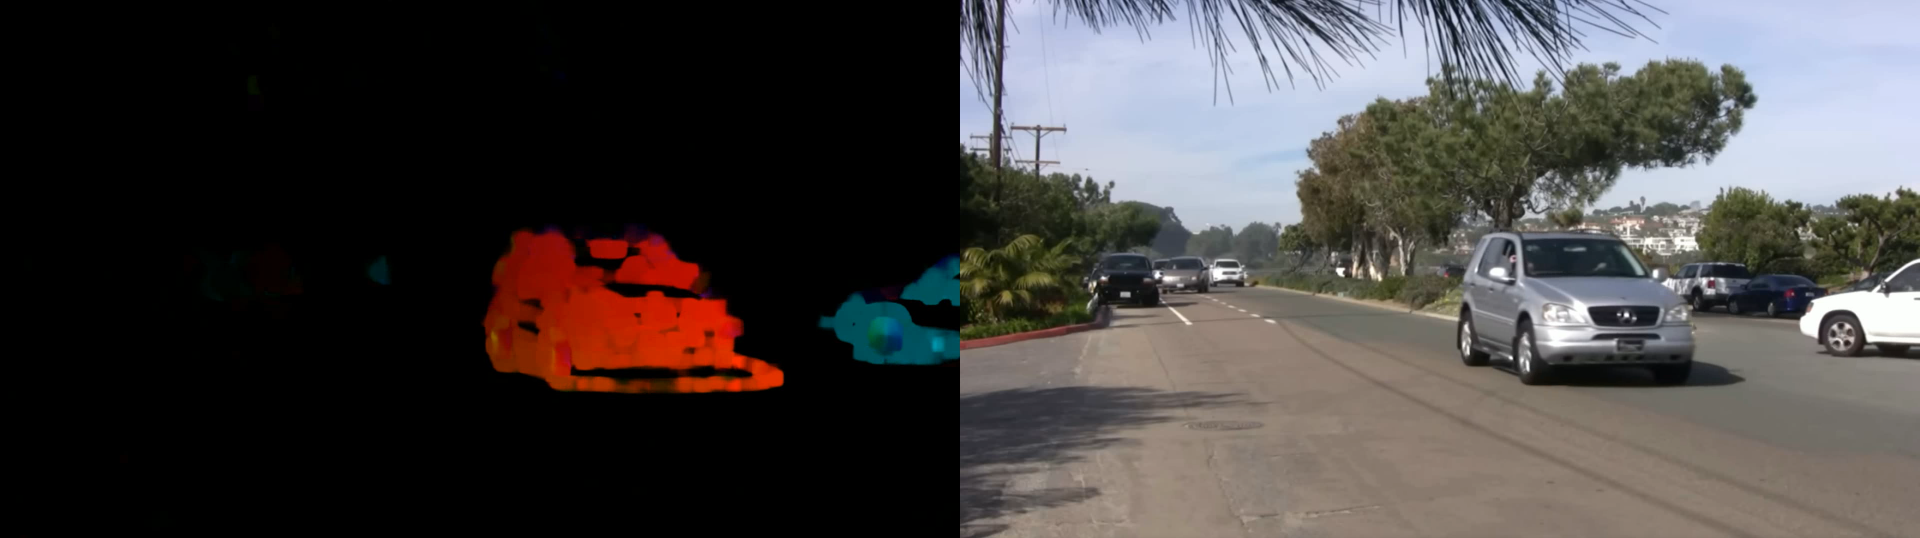
\includegraphics[width=0.9\linewidth]{_images/farneback_cars1}
			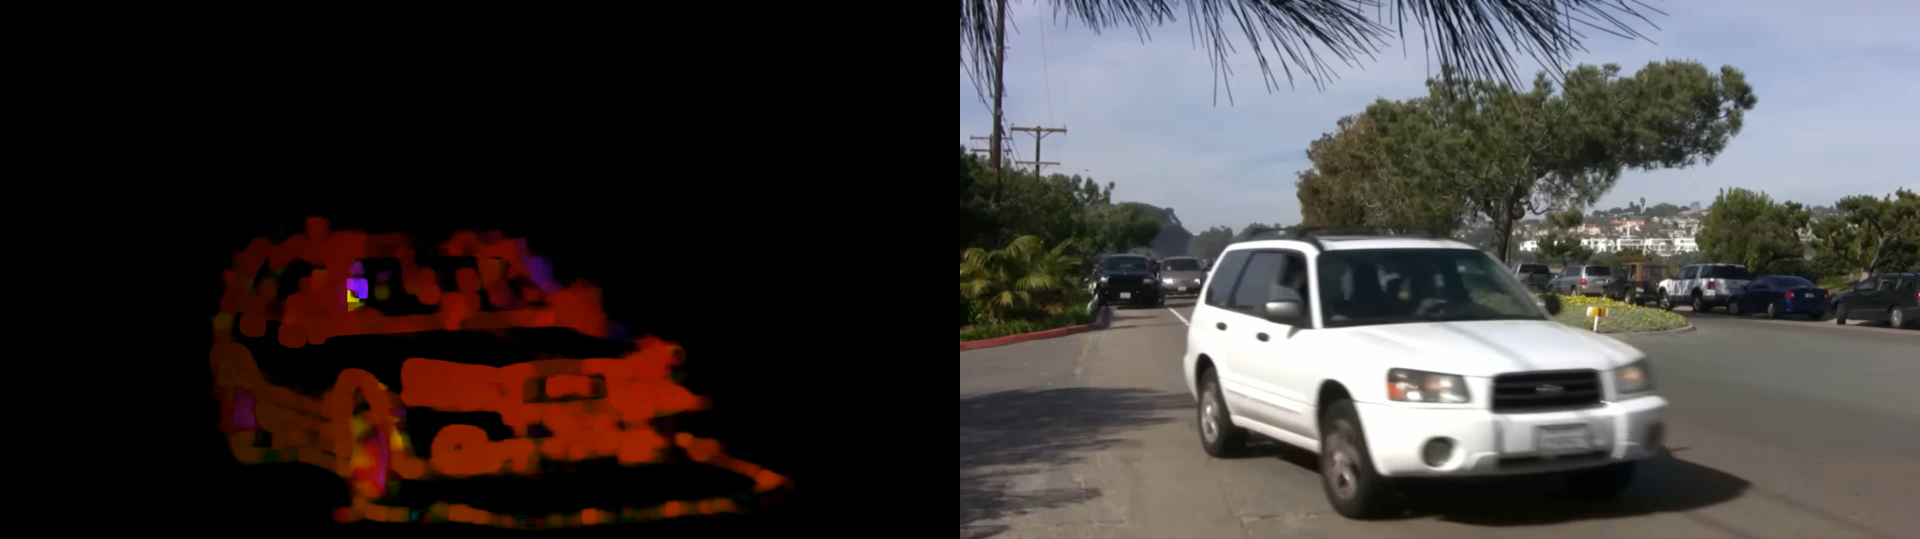
\includegraphics[width=0.9\linewidth]{_images/farneback_cars2}
			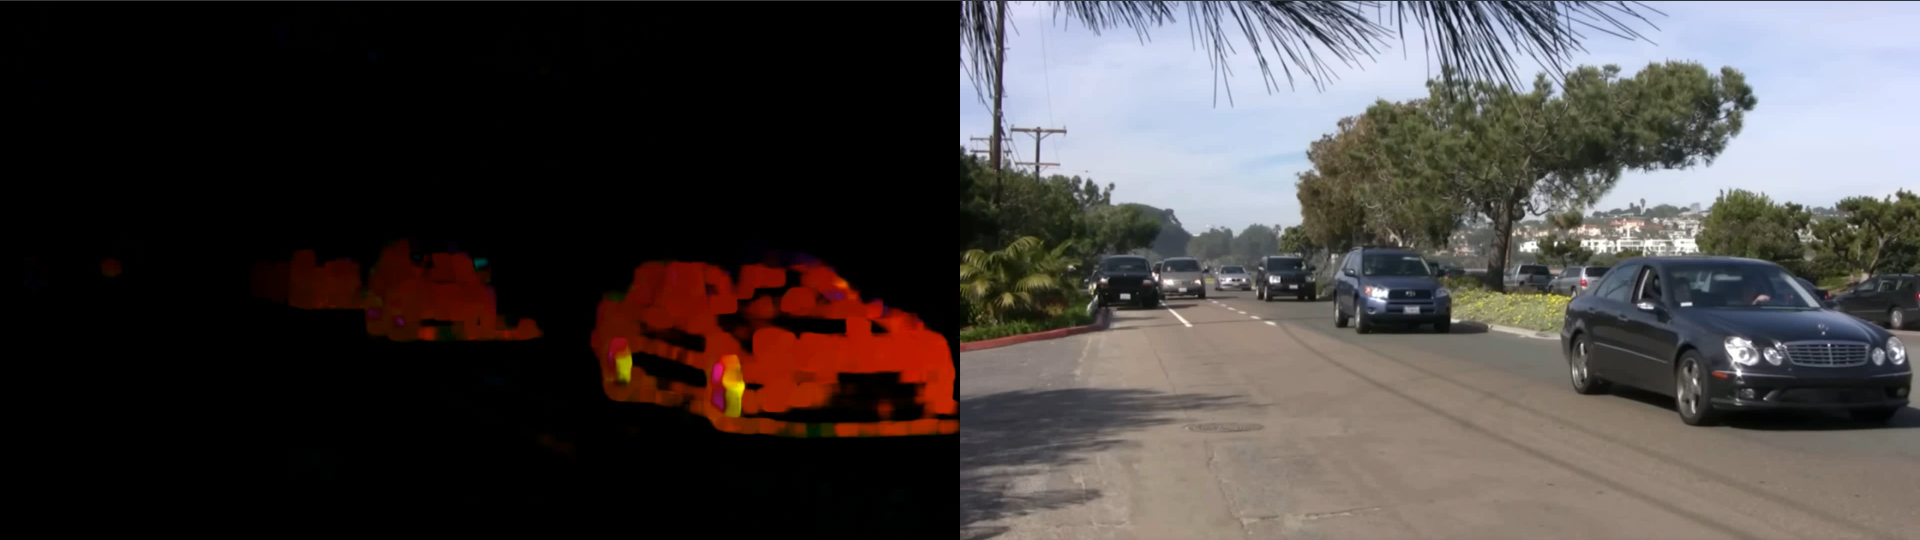
\includegraphics[width=0.9\linewidth]{_images/farneback_cars3}
			\caption{Output of Farneback Dense Optical FLow Algorithm applied to video of cars driving by.}
			\label{fig:farnebackcars1}
		\end{figure}
		
		\item RLOF\\
		The code that uses the RLOF instead of the Farneback OF is pretty similar. The single thing that changes is the DOF call. Thanks to OpenCV this has been made relatively simple. I myself did a mistake which led to much debugging and messing around. A deeper explanation can be found in in the section \ref{Discussion}. 
		
\begin{lstlisting}[language=python]
flow = cv.optflow.calcOpticalFlowDenseRLOF(frame1, frame2, None)
\end{lstlisting}
The above line of code is the single most important line of the code. Everything else is just there for reading the video as a sequence of images and convert the resulting images to more informative ones. Also there is some code for storing and display.
A important note is that RLOF can work with RGB images whilst Farneback only supports grayscale images. I didn't set any of the values so the default values were set. This is important as the resulting videos seem to be good.
		
		\begin{figure}[H]
			\centering
			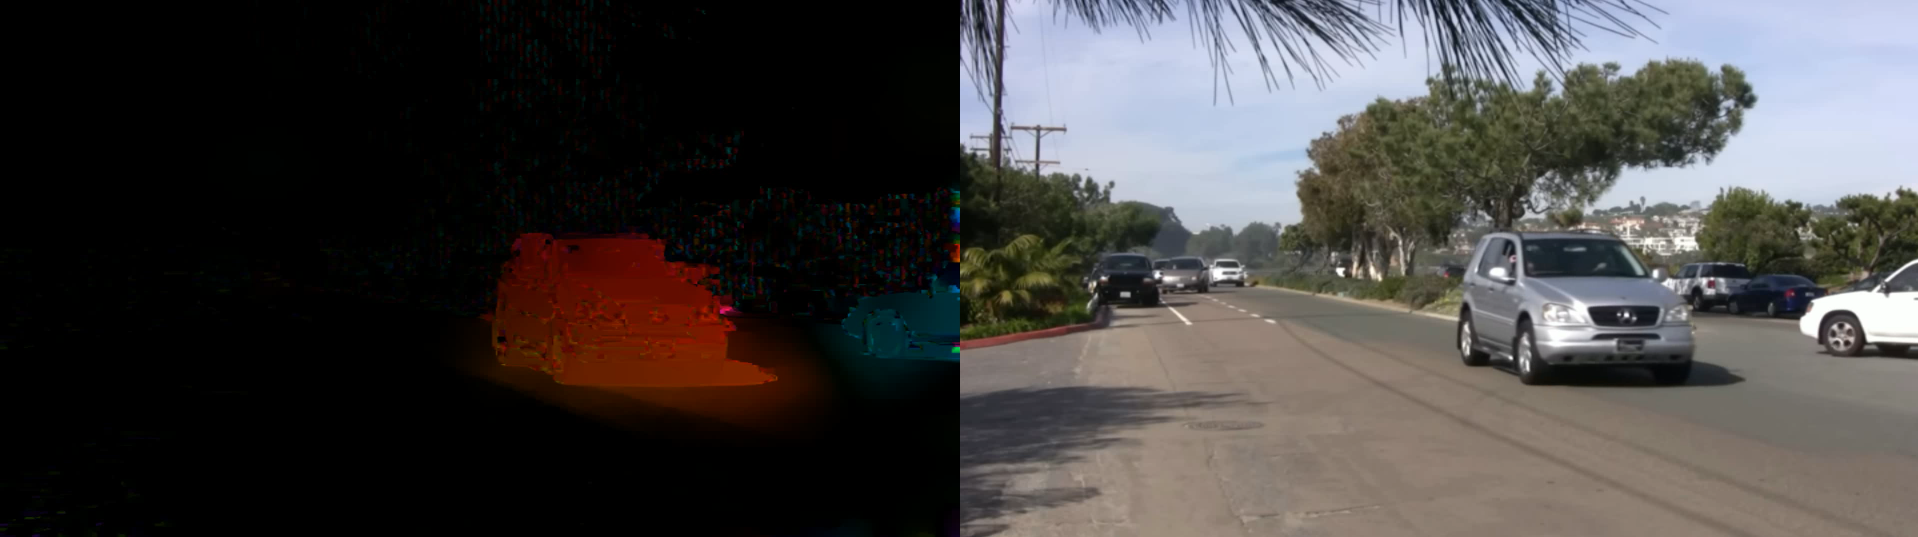
\includegraphics[width=0.9\linewidth]{_images/RLOF_cars1}
			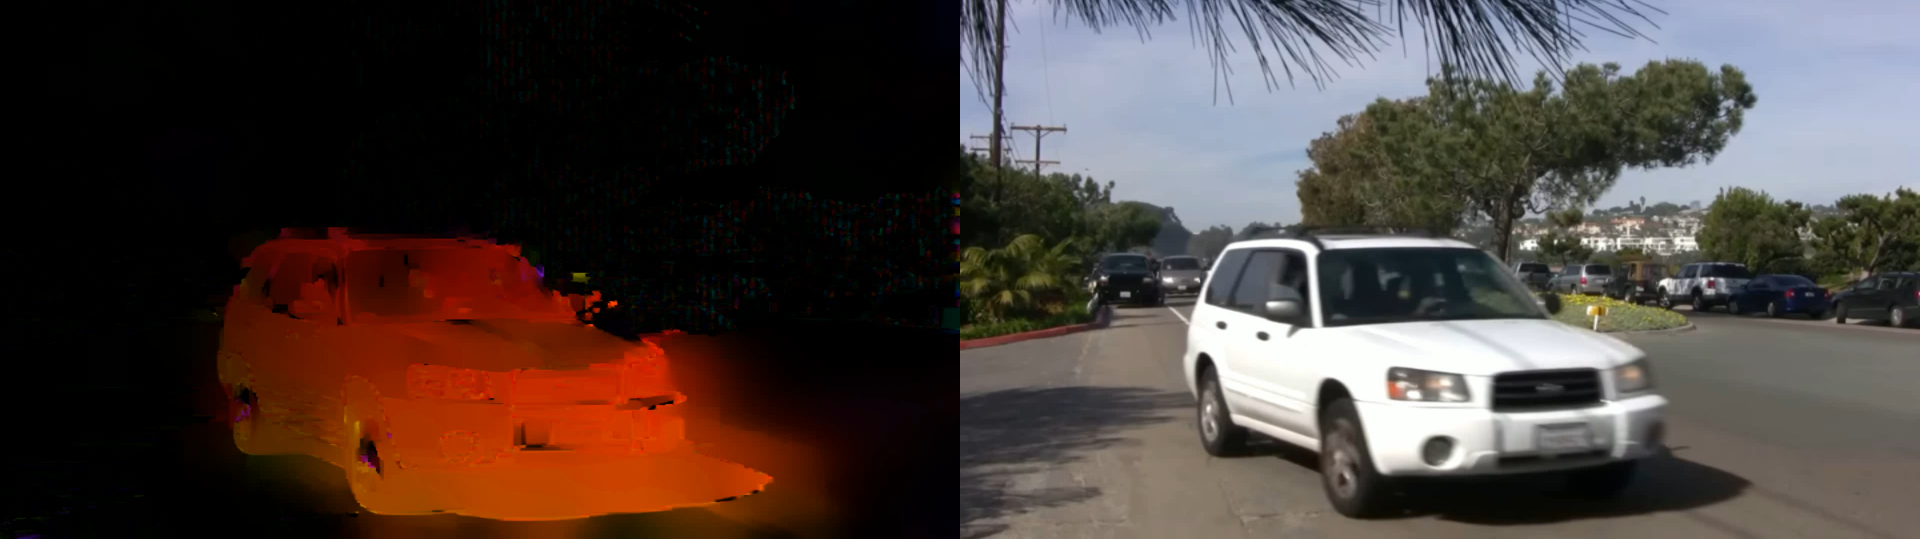
\includegraphics[width=0.9\linewidth]{_images/RLOF_cars2}
			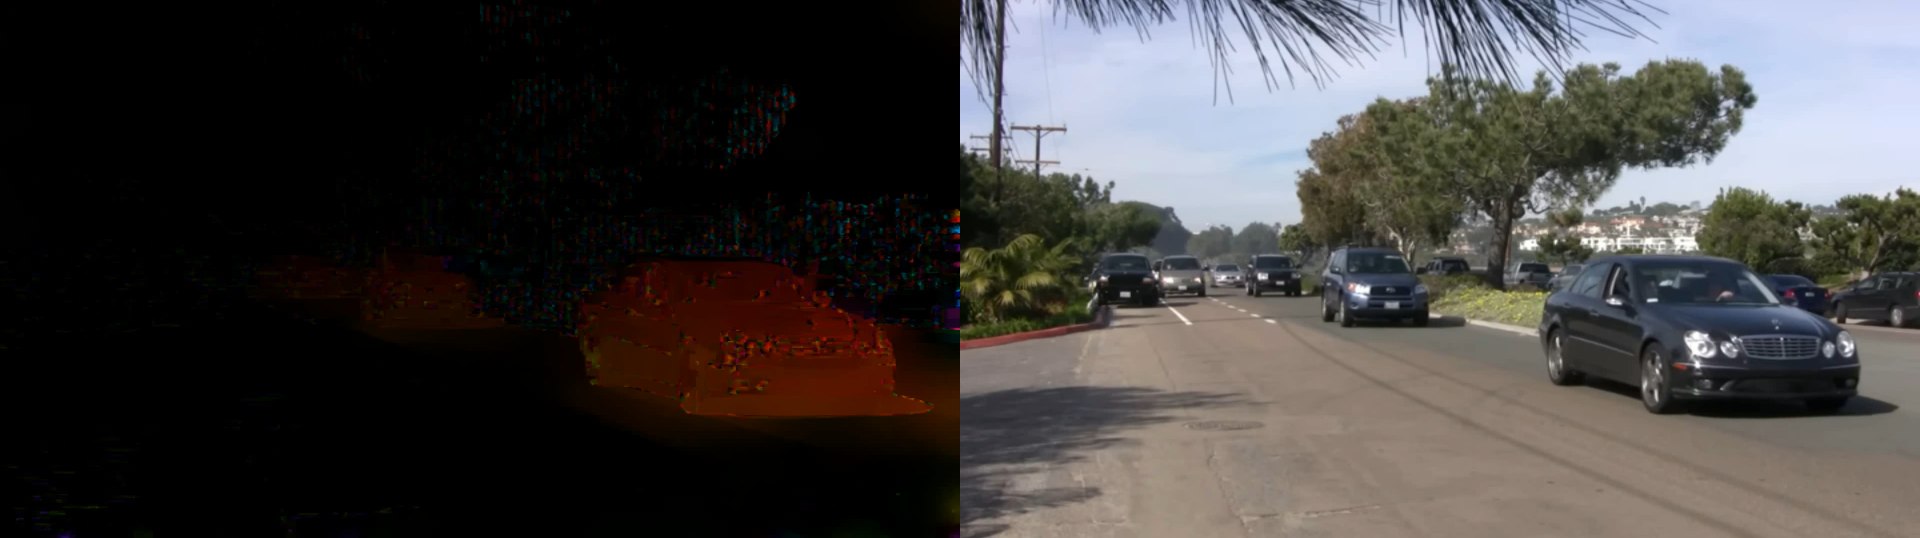
\includegraphics[width=0.9\linewidth]{_images/RLOF_cars3}
			\caption{Output of RLOF Algorithm applied to video of cars driving by.}
			\label{fig:rlofcars1}
		\end{figure}
	\end{enumerate}
\textbf{Evaluation and discussion of the dense OF algorithms}
After running both of these algorithms which took a while, because they have to calculate the differences of two images with both in this case having $\sim$ 400.000 pixels each. The output of the RLOF seems to be much better pronounced with a higher level of detail. Farneback for example has a problem with reflective surfaces or see through surfaces like the windows in the images. Also with large homogenous surfaces like the hoods of the cars. RLOF seems to be a good alternative to Farneback. This is supported by the observation that both algorithms had a similar runtime. I haven't measured it but they've seemed really close.
\end{enumerate}



\newpage
	\section*{Task 3}
	Report on how your solution was implemented (including equations) and the algorithms you
	followed to solve the assignment. Include snippets (only interesting parts of the code) and
	snapshots of frames regarding the optical flow output solutions. Comment on the results and how
	the algorithms compare.\\\\
	
(6 points) Motion analysis using spatiotemporal filters. Use the video from question 2 and
create a program that analyze motion using spatiotemporal filtering:

\begin{enumerate}[a.]
	\item Use the following spatiotemporal 9-tap filters from the classical work of Freeman
	and Adelson (1991):
	\begin{itemize}
		\item f1 = {0.0094,0.1148,0.3964,-0.0601,-0.9213,-0.0601,0.3964,0.1148,0.0094}
		for the x dimension.
		\item f2 = {0.0008, 0.0176, 0.1660, 0.6383, 1.0, 0.6383, 0.1660, 0.0176, 0.0008}
		for the t dimension.
	\end{itemize}
	Note: values taken from Appendix H in \href{http://people.csail.mit.edu/billf/www/papers/steerpaper91FreemanAdelson.pdf}{original paper Freeman and Adelson}
	\item Compare the spatiotemporal solutions with the Dense Optical flow solutions from
	question 2b and comment on how they compare.
	\item Your output should be a sequence of frames (video) such as the following (only the
	person and the plant leafs because of air conditioning are moving).
	\begin{figure}[H]
		\centering
		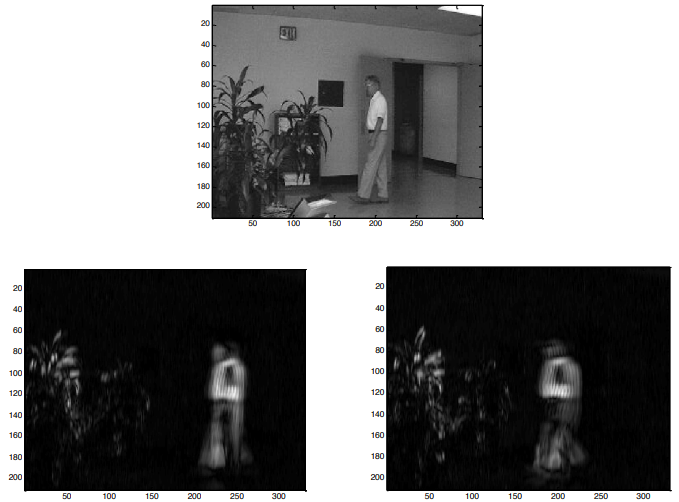
\includegraphics[width=0.7\linewidth]{_images/instructions3c}
		%\caption{}
		\label{fig:instructions2c}
	\end{figure}
	In summary, we extract the objects in motion\\
	Note that you may (or maybe not) have problems with memory (video is a sequence
	of many images), you should be able to handle that.
\end{enumerate}

I've implemented 2 algoithms which are similar to each other. I will explain the simple or primitive one first.\\

At first we begin by loading 9 images (dependant on the size of the temporal filter) into a ringbuffer. All of those images are convolved while loading.\\
\begin{align}
	I_{convolved_x} = I * f_x
\end{align}

As the filter is a separable 1D filter we have to apply it again, but this time transpose it.

\begin{align}
	I_{convolved_{xy}} = I_{convolved_x} * f_x^T
\end{align}

Now we have a full buffer with space convolved images.\\
These images have to be convolved in the time axis. Here our mentioned ringbuffer will be handy.

\begin{align}
	I_{convolved_{xyt}}(x,y) = \sum_{f = 0}^{f_t} I_{convolved_{xy}}(x,y,t) \cdot f
\end{align}

Where $I_{convolved_{xy}}(x,y,t)$ is the x-th row and y-th column pixel of the t-th image from the buffer.


In terms of code I've made functions for reading the images from the stream and for the application of the separable convolution.

\begin{lstlisting}[language=python]
def read_grayscale_img(cap):
ret, img = cap.read()
if not ret:
print('Stream ended!')
cap.release()
sys.exit(0)
img = cv.cvtColor(img, cv.COLOR_BGR2GRAY)
return img

def apply_separable_filter(img, filter):
img = cv.filter2D(img, -1, filter)
return cv.filter2D(img, -1, filter.T)
\end{lstlisting}

The convolution is calculated in a for loop and looks like this.

\begin{lstlisting}[language=python]
for i, time_filter in enumerate(filter_t):
	t_convolved += imgs[i] * time_filter
\end{lstlisting}

Here the entire image is multiplied by the value of the t-th element of the filter, so we calculate the entire image value not pixel by pixel.\\
Interesting addition, Python actually doesn't provide a ringbuffer per default, but we can utilize the generic list, as it implements pop with the possibility to select an element to pop.
\\


\begin{figure}[H]
	\centering
	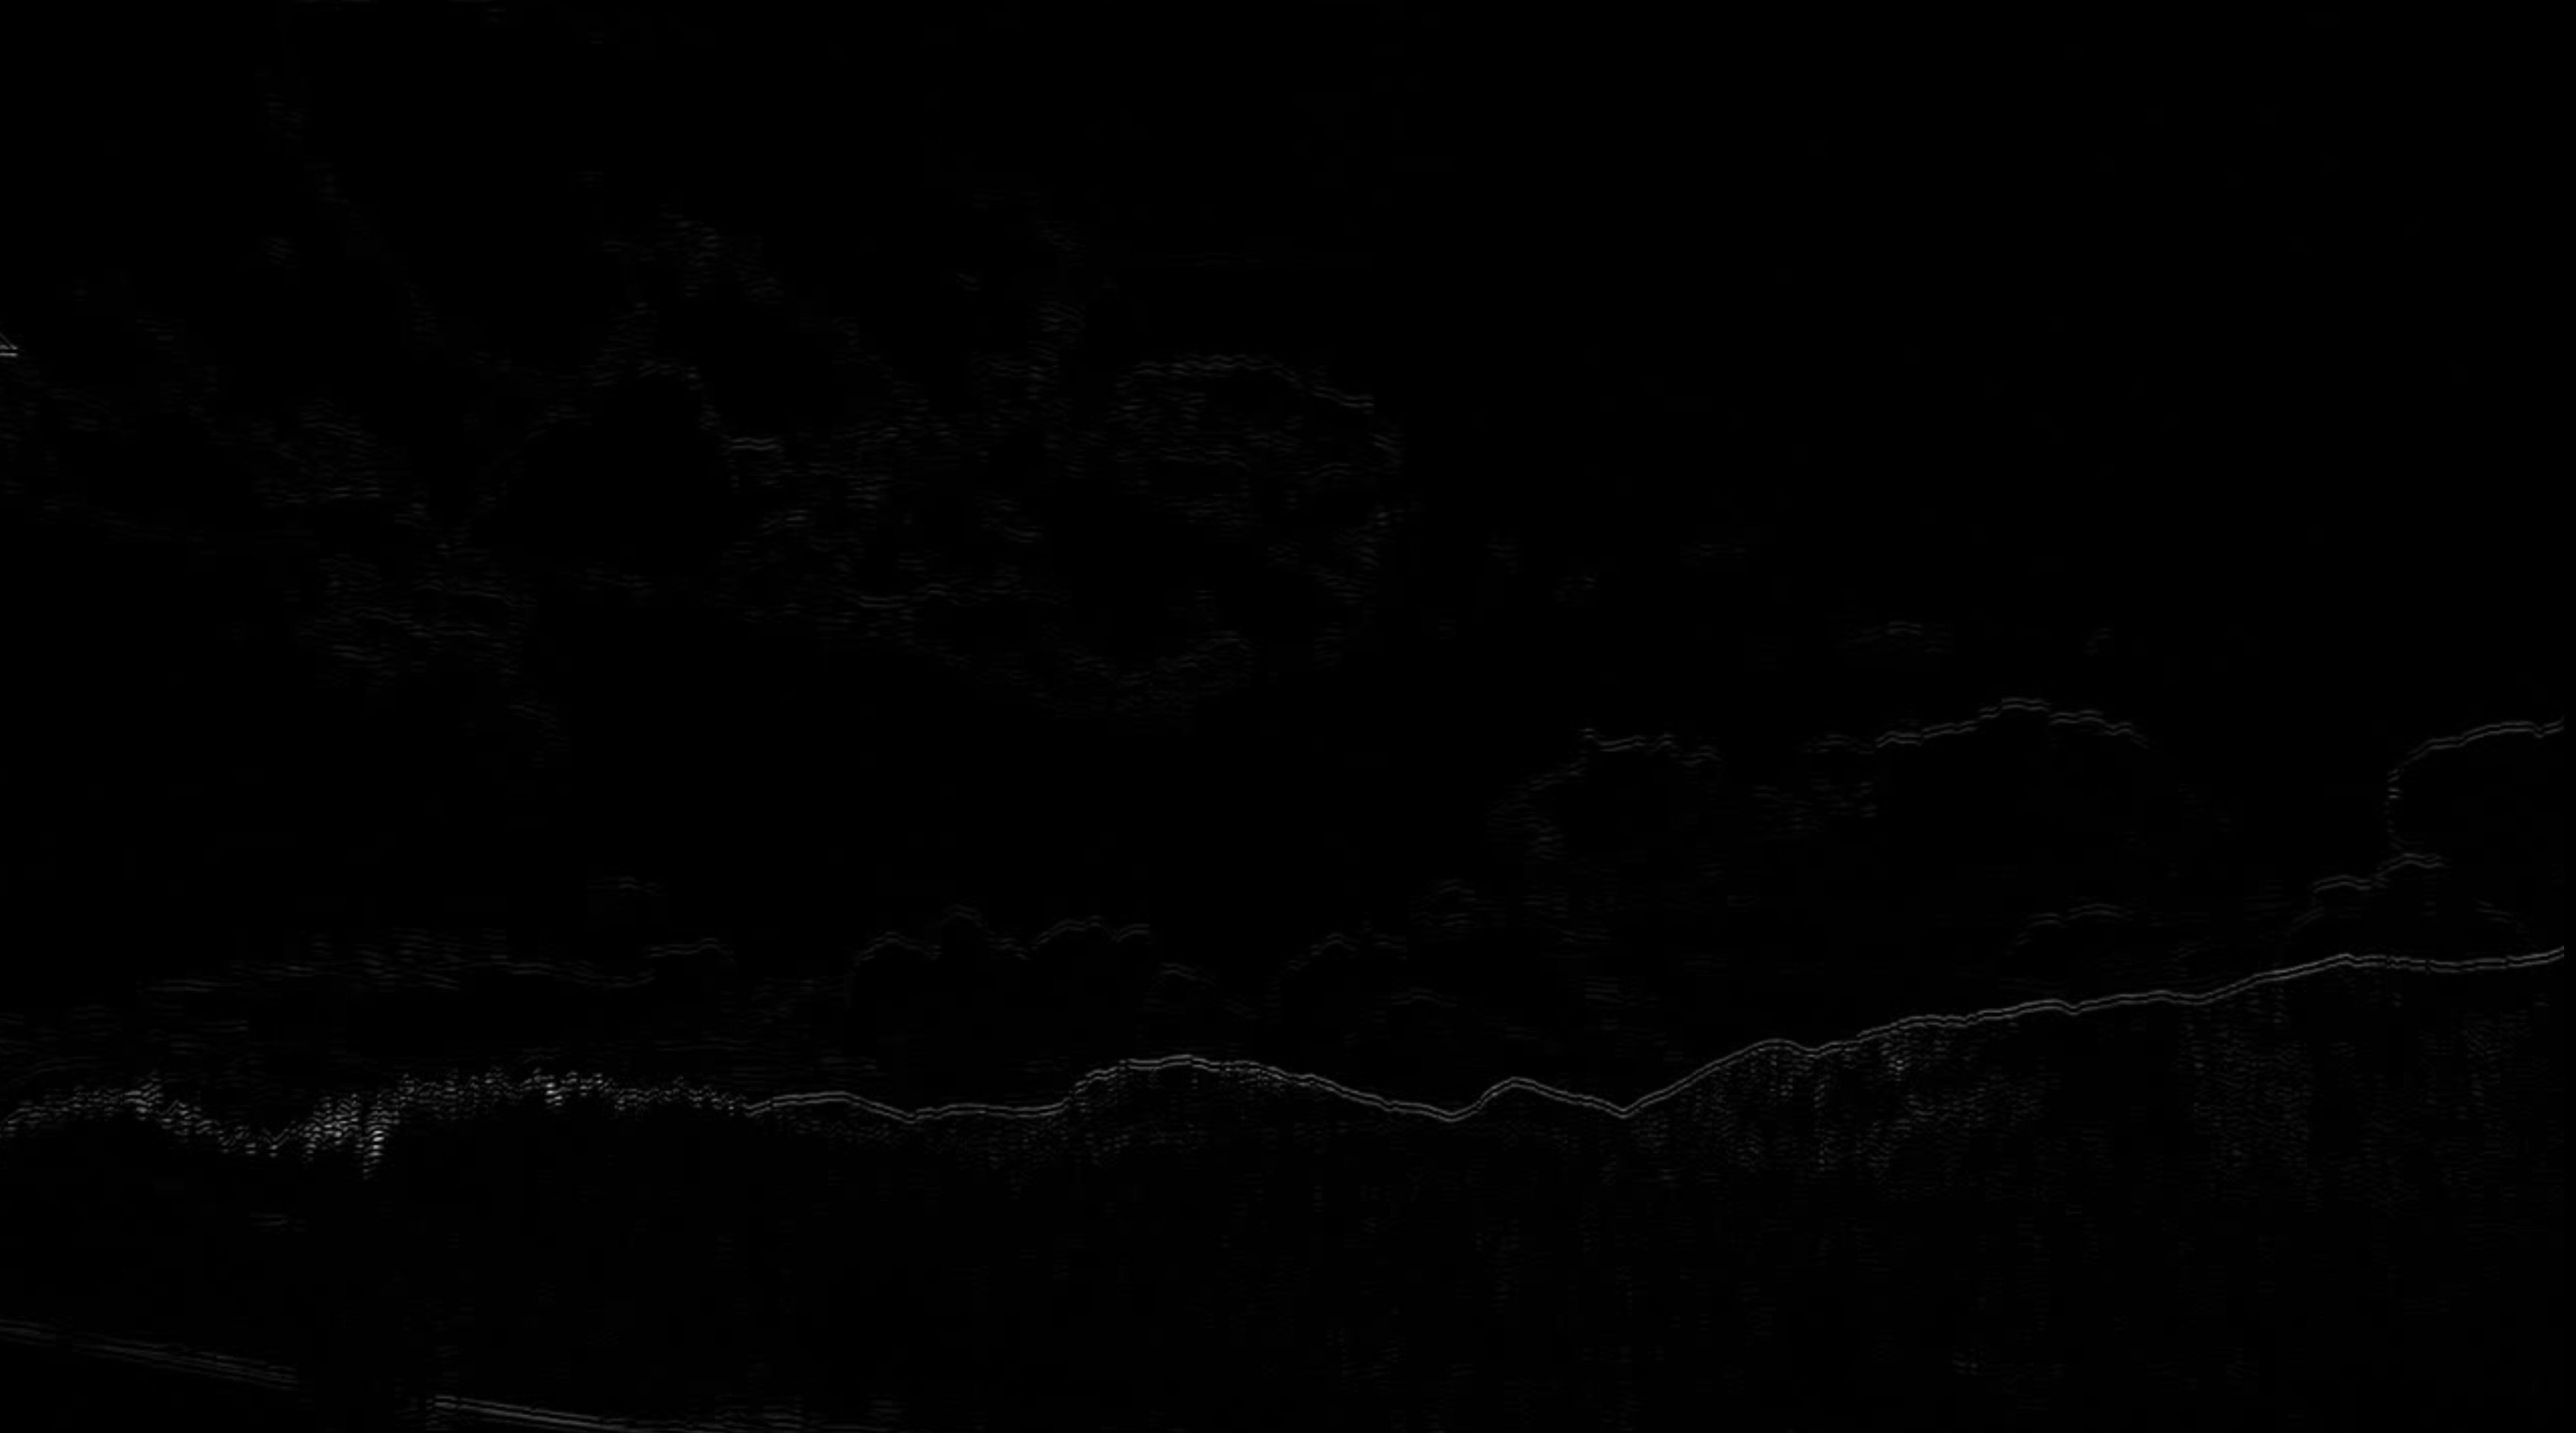
\includegraphics[width=0.7\linewidth]{_images/spatiotemporal_first1}
	\caption{First implementation result on clouds footage.}
	\label{fig:spatiotemporalfirst1}
\end{figure}
\begin{figure}[H]
	\centering
	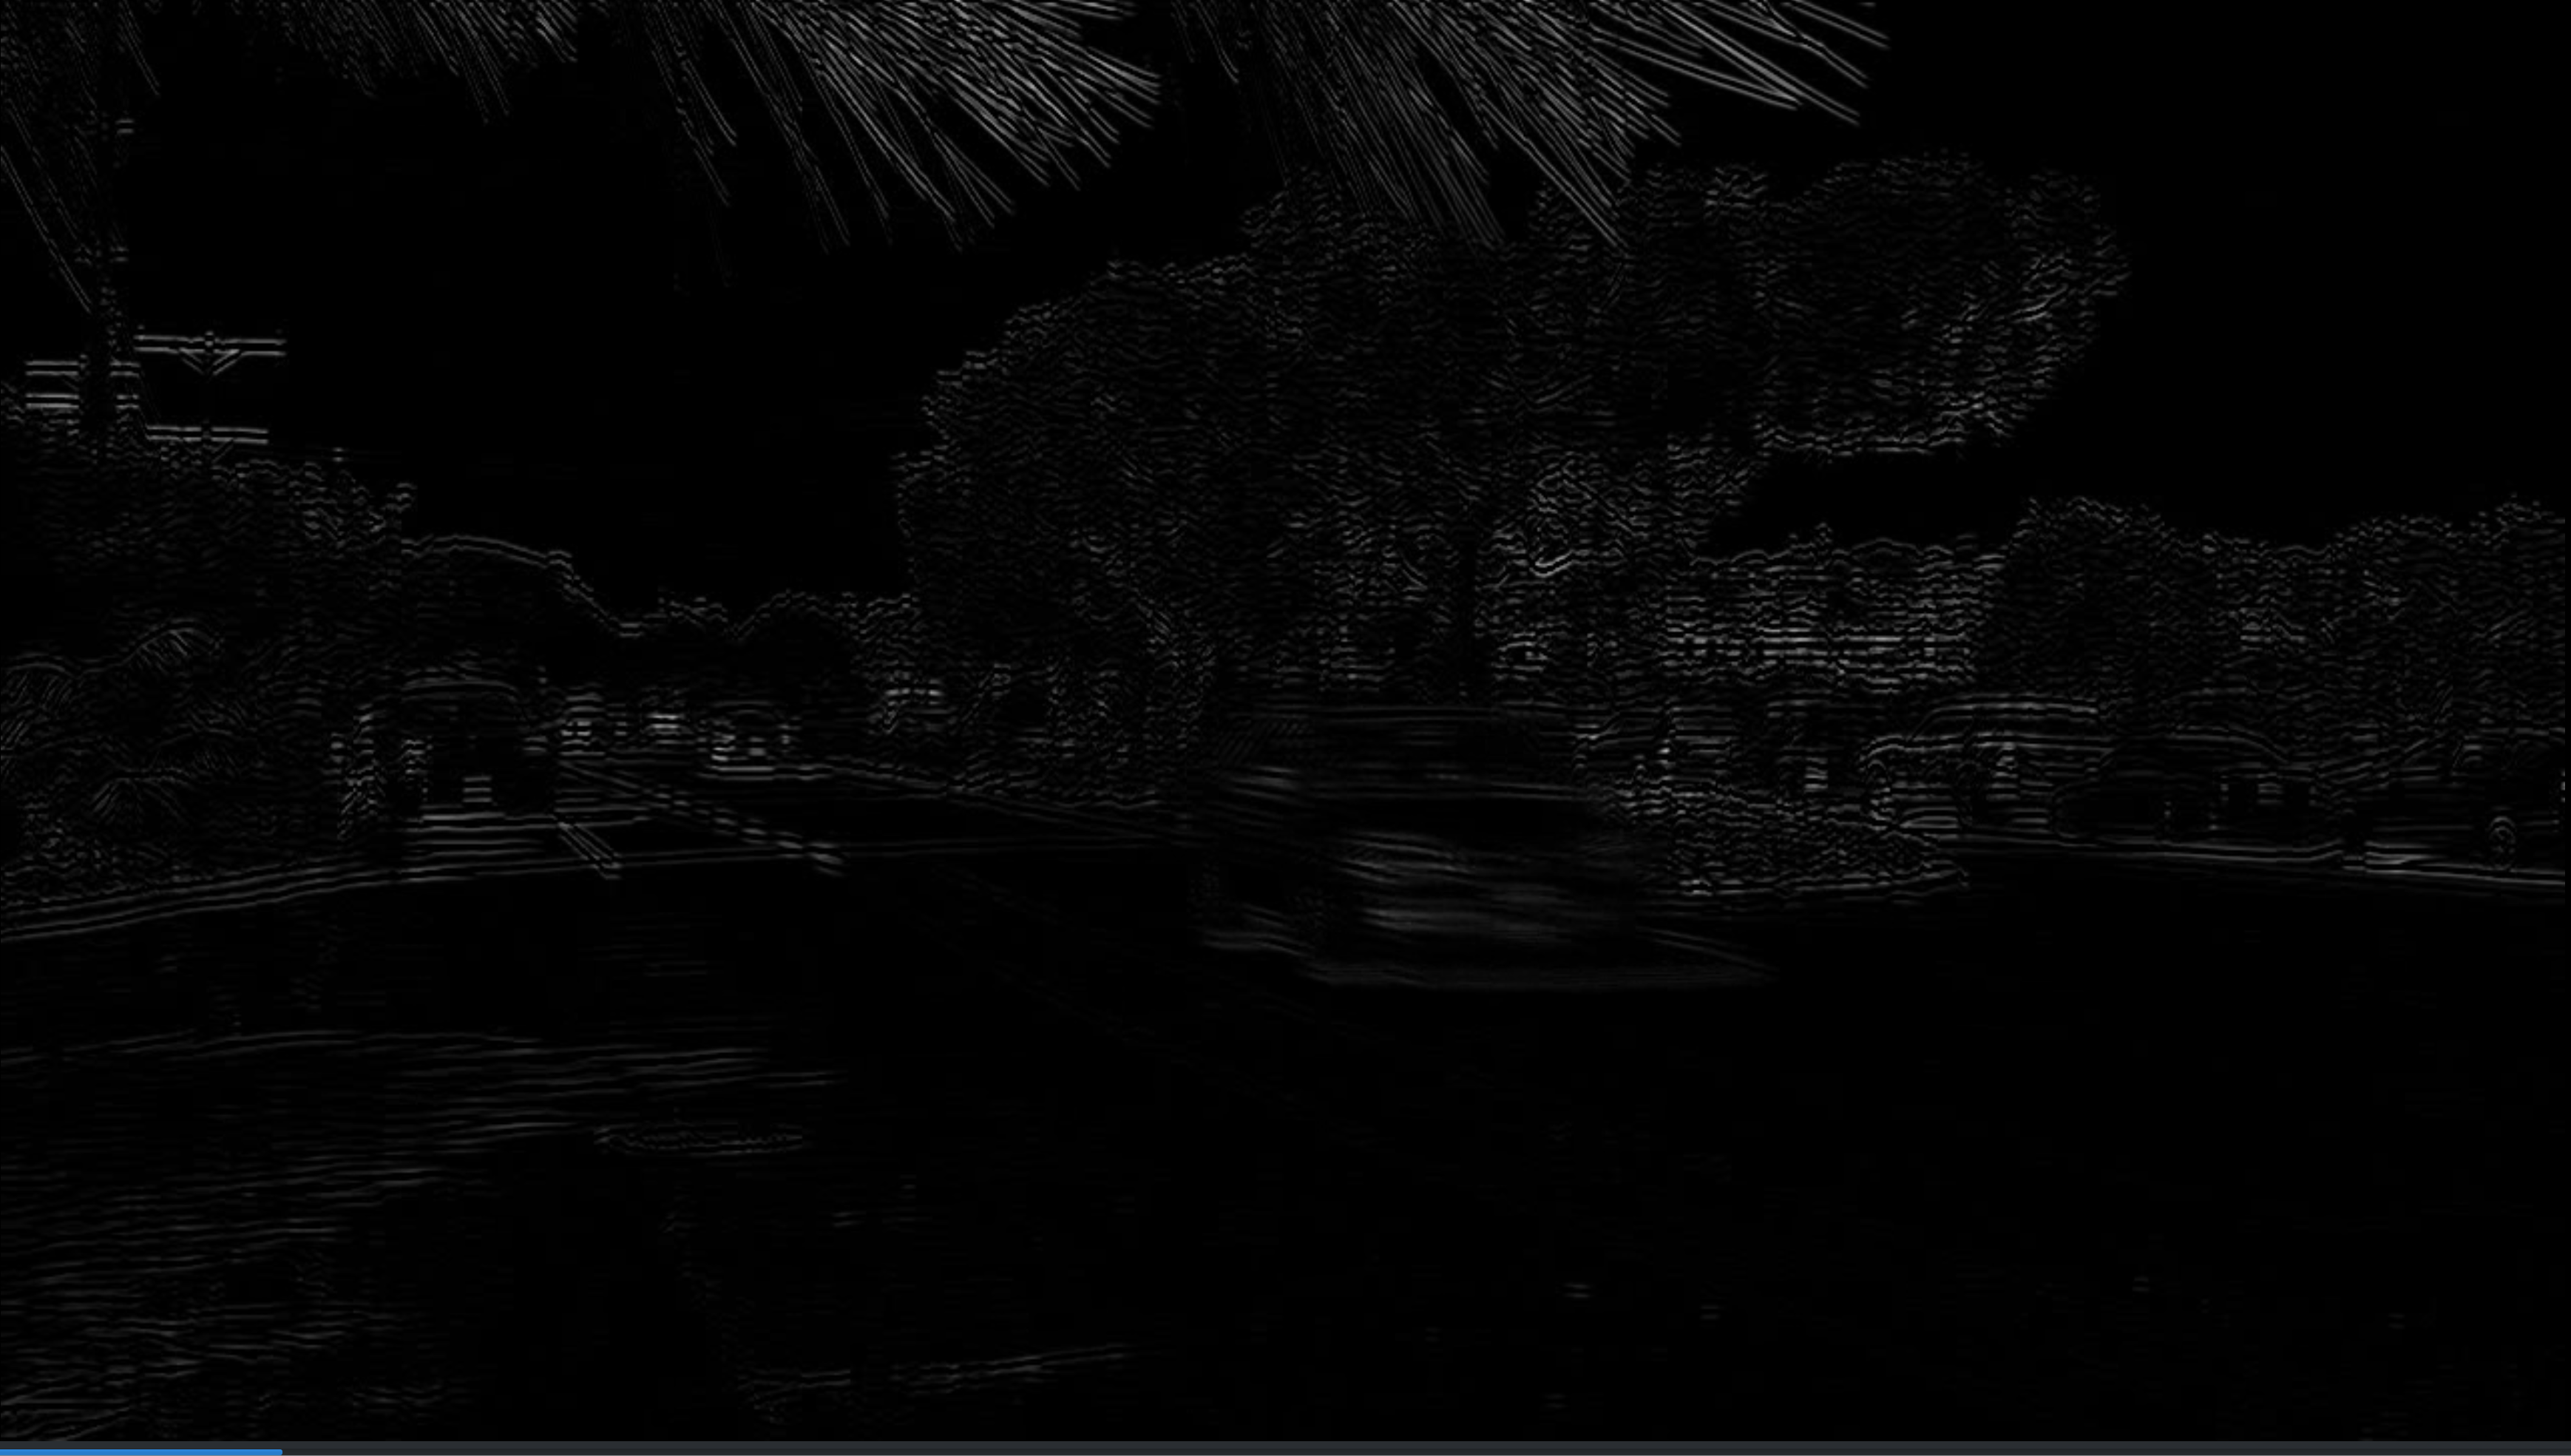
\includegraphics[width=0.7\linewidth]{_images/spatiotemporal_first2}
	\caption{First implementation result on cars footage.}
	\label{fig:spatiotemporalfirst2}
\end{figure}
The results of this implementation are a bit disappointing in my opinion.\\
I've then tried to remove the static parts of the image by subtracting the average of each pixel.

\begin{align}
	I_{avg}(x,y) = \frac{1}{t} \sum_{i=0}^{t} I(x,y,i)
\end{align}

Where $t$ is each image on the time axis of the video.
After calculating the average image we can go ahead and subtract a smoothed version of it on every newly loaded image.
\\
The rest is similar to the first version.

\begin{figure}[H]
	\centering
	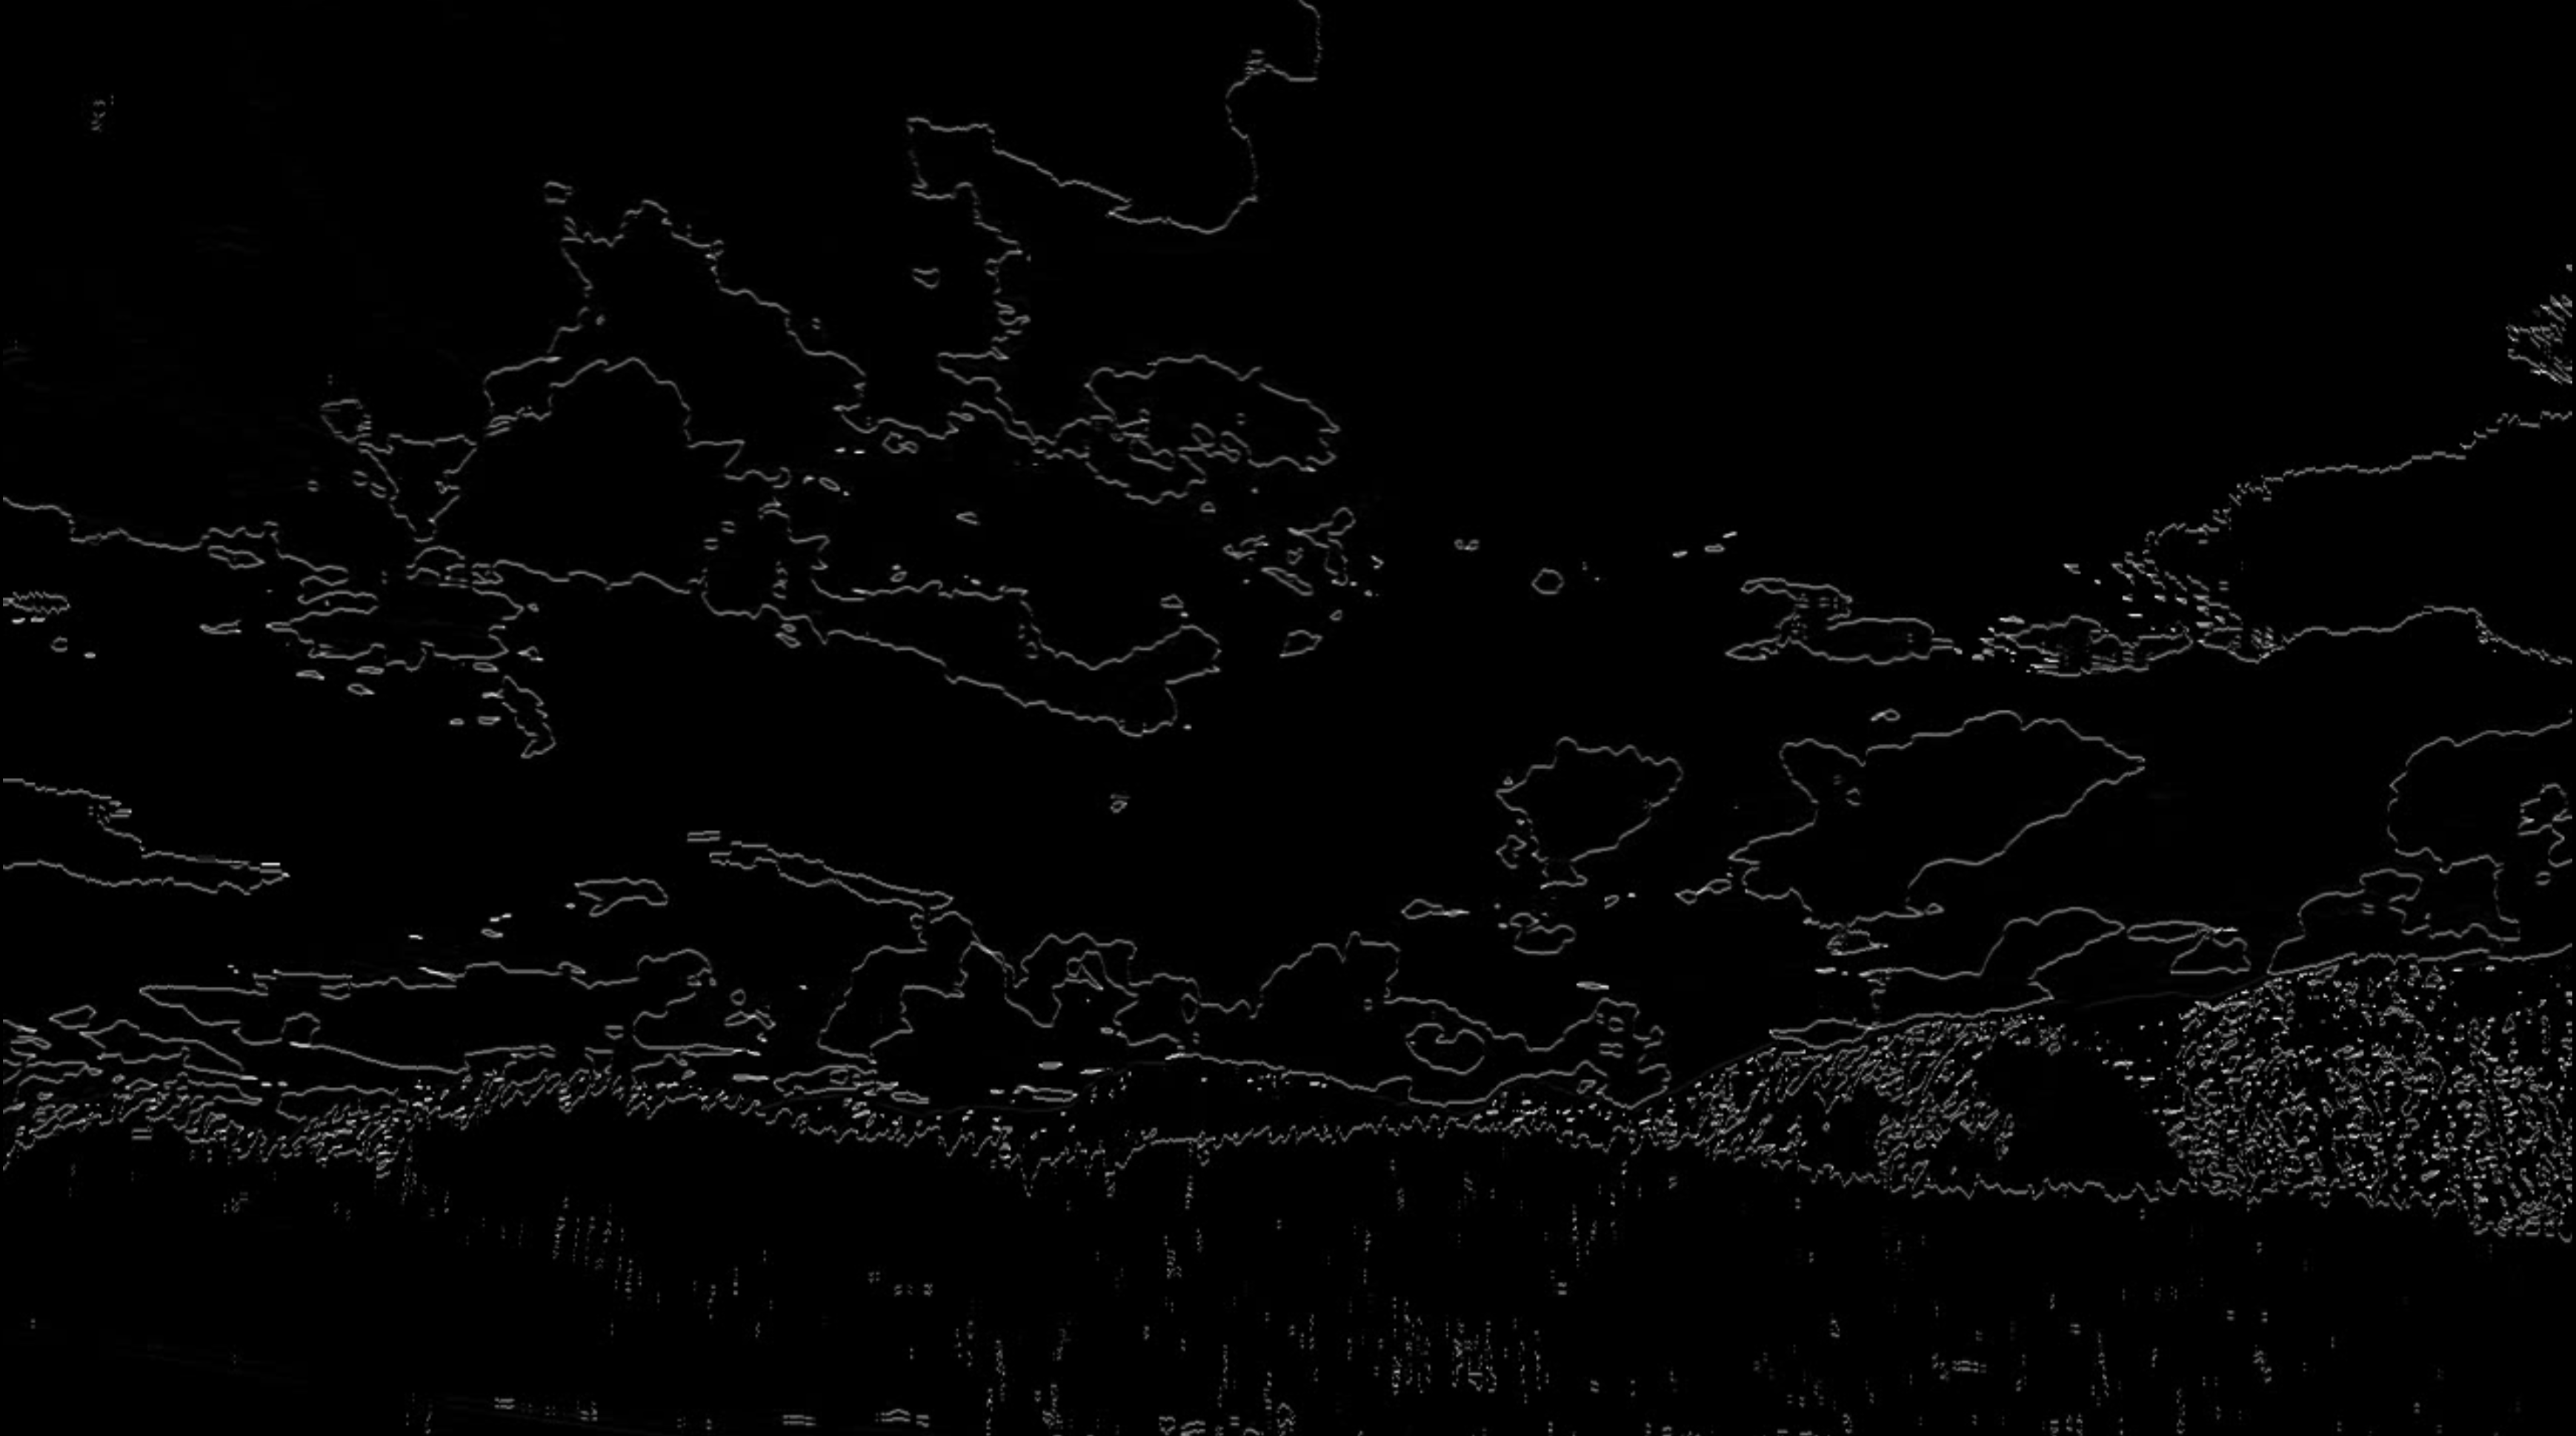
\includegraphics[width=0.7\linewidth]{_images/spatiotemporal_snd1}
	\caption{First implementation result on clouds footage.}
	\label{fig:spatiotemporalsecond1}
\end{figure}

\begin{figure}[H]
	\centering
	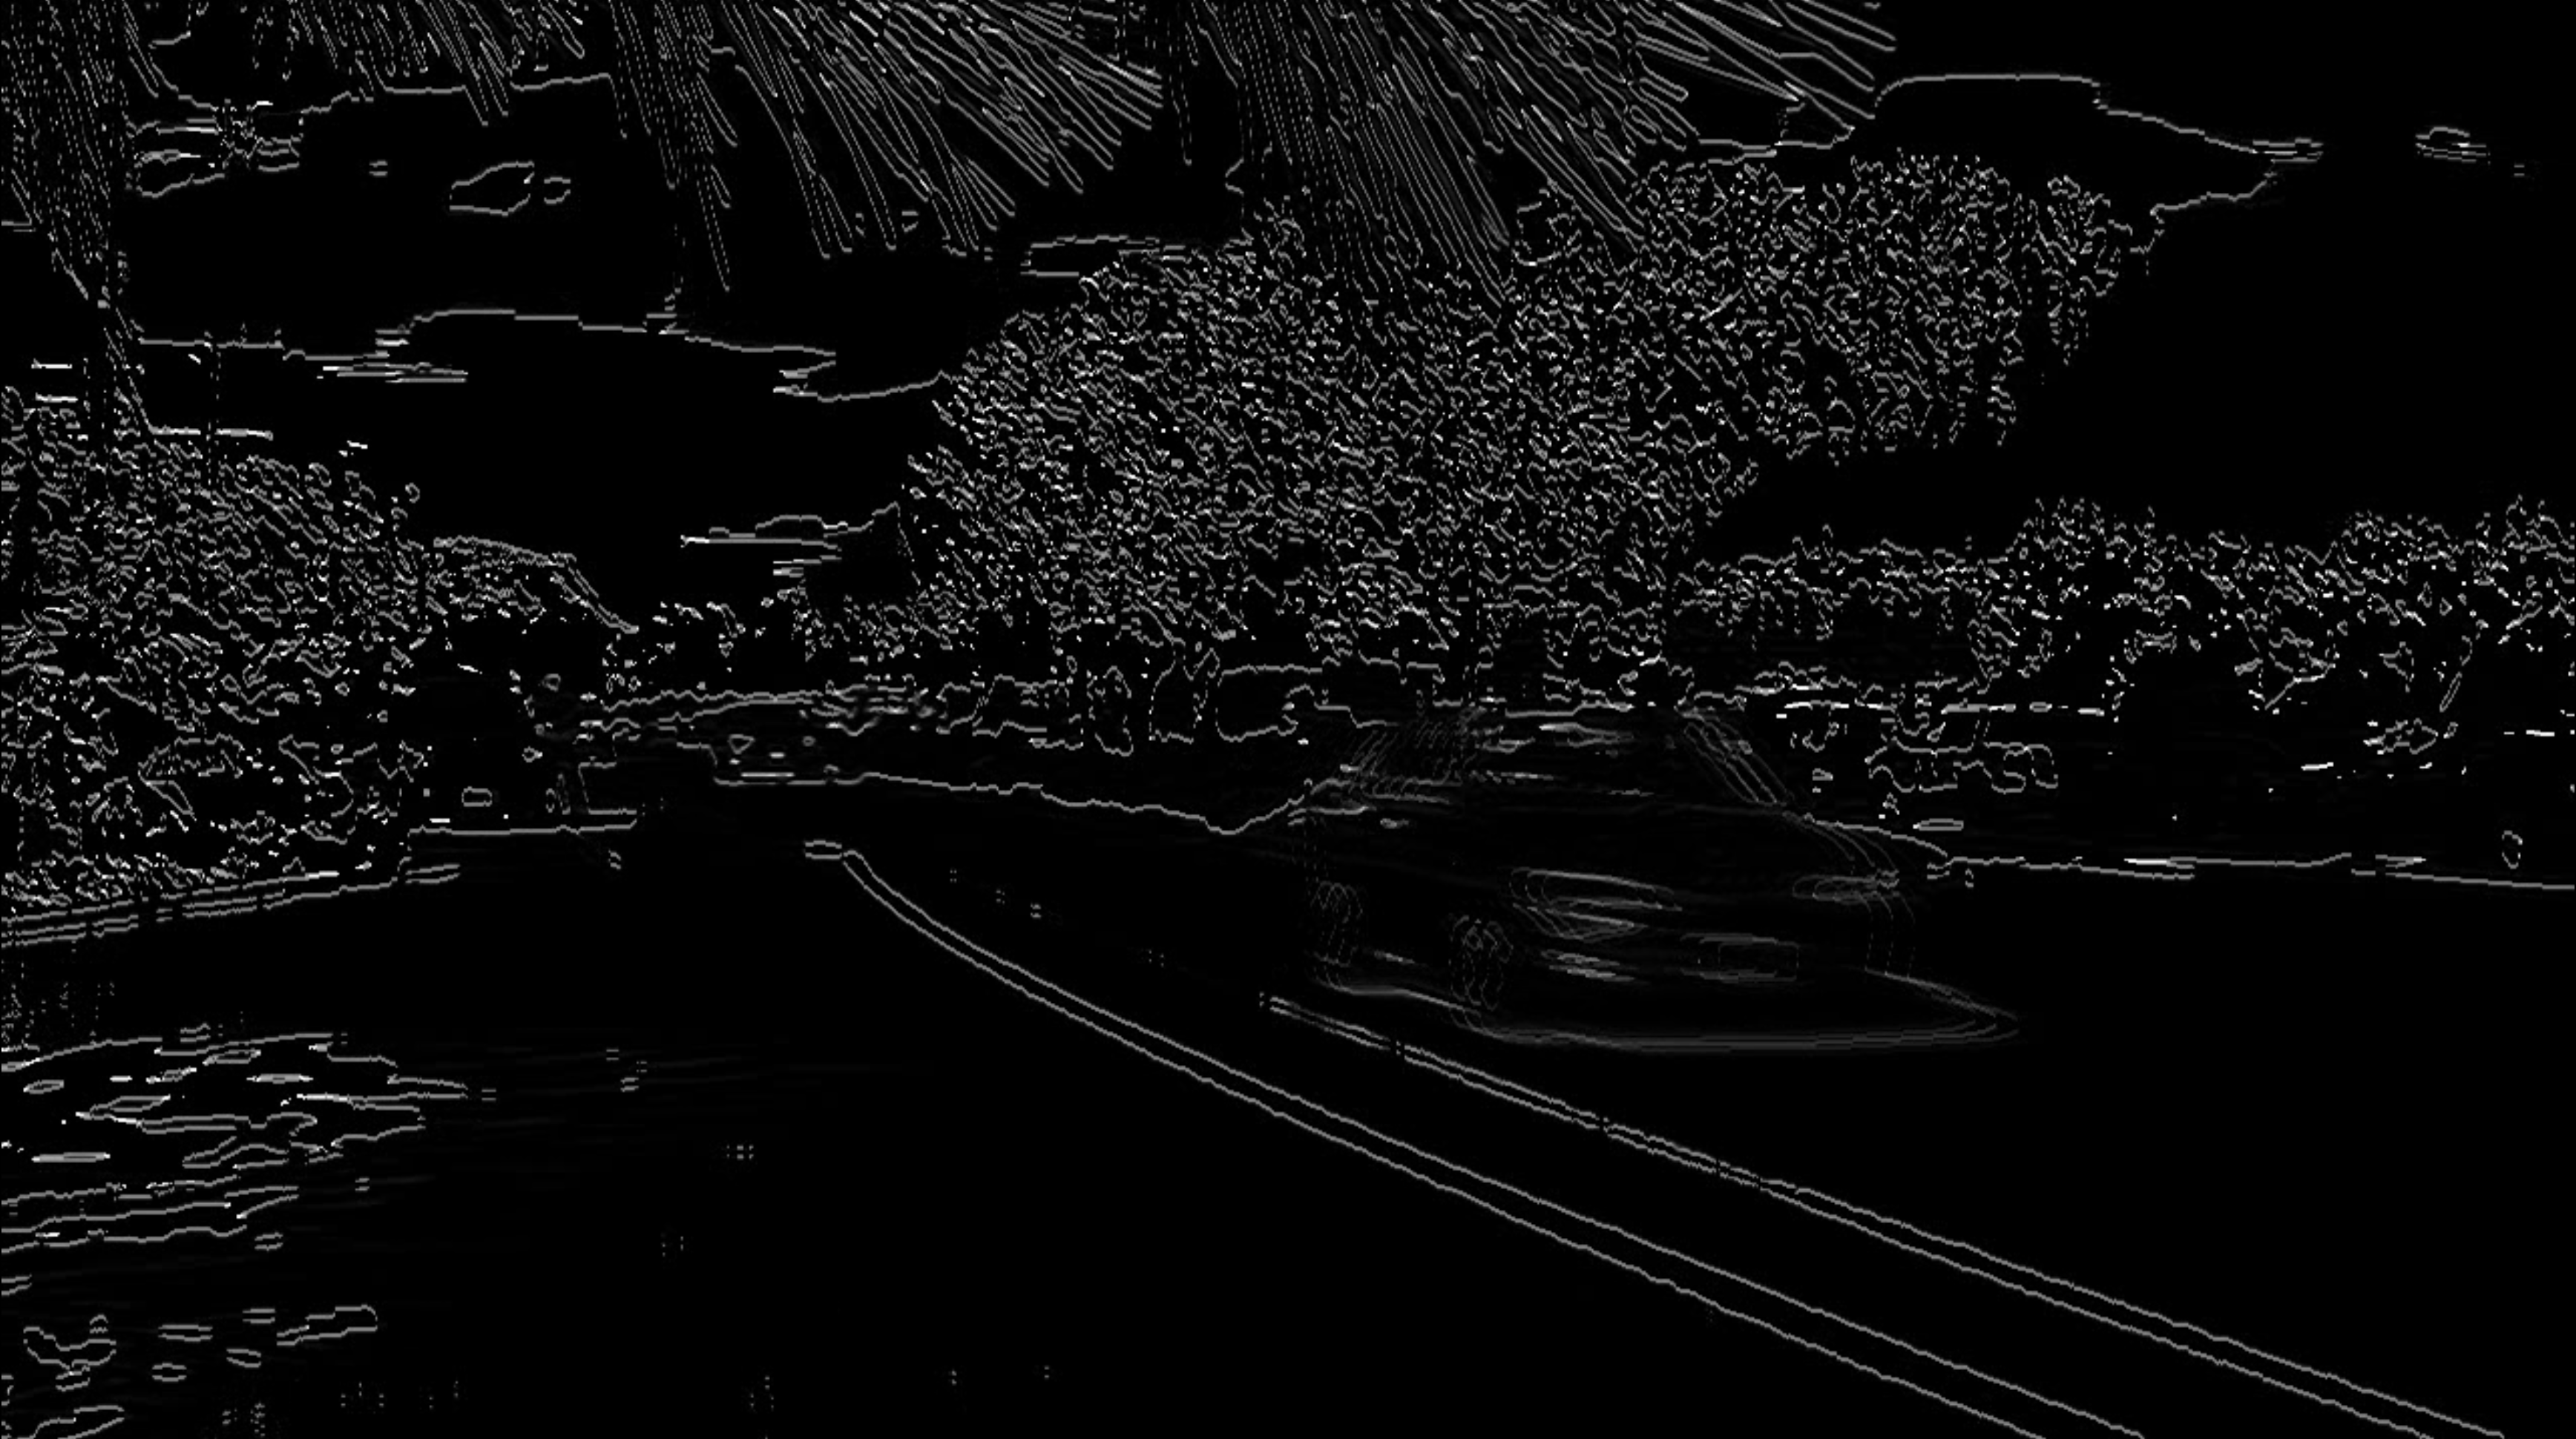
\includegraphics[width=0.7\linewidth]{_images/spatiotemporal_snd2}
	\caption{First implementation result on clouds footage.}
	\label{fig:spatiotemporalsecond2}
\end{figure}

With the averages looking like the following.

\begin{figure}[H]
	\centering
	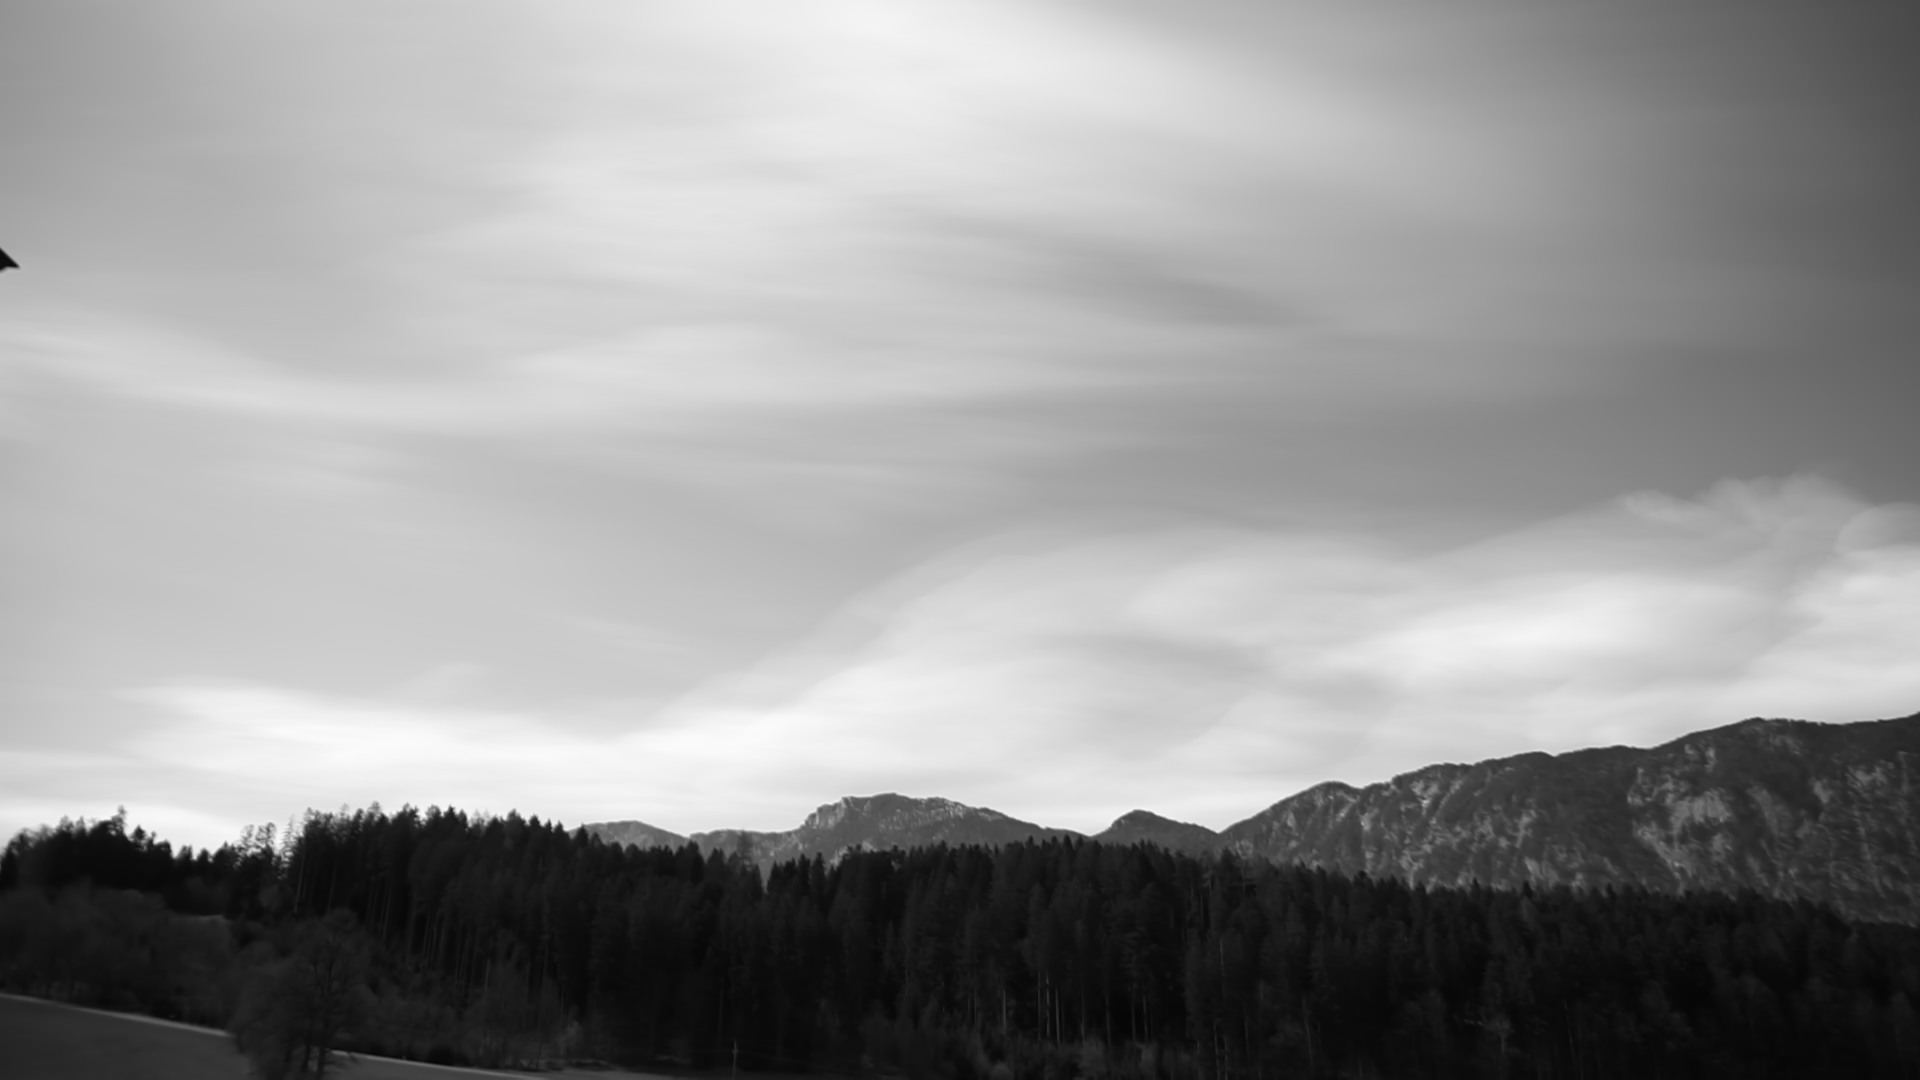
\includegraphics[width=0.7\linewidth]{_images/averageImage_spatiotemporalClouds3.png}
	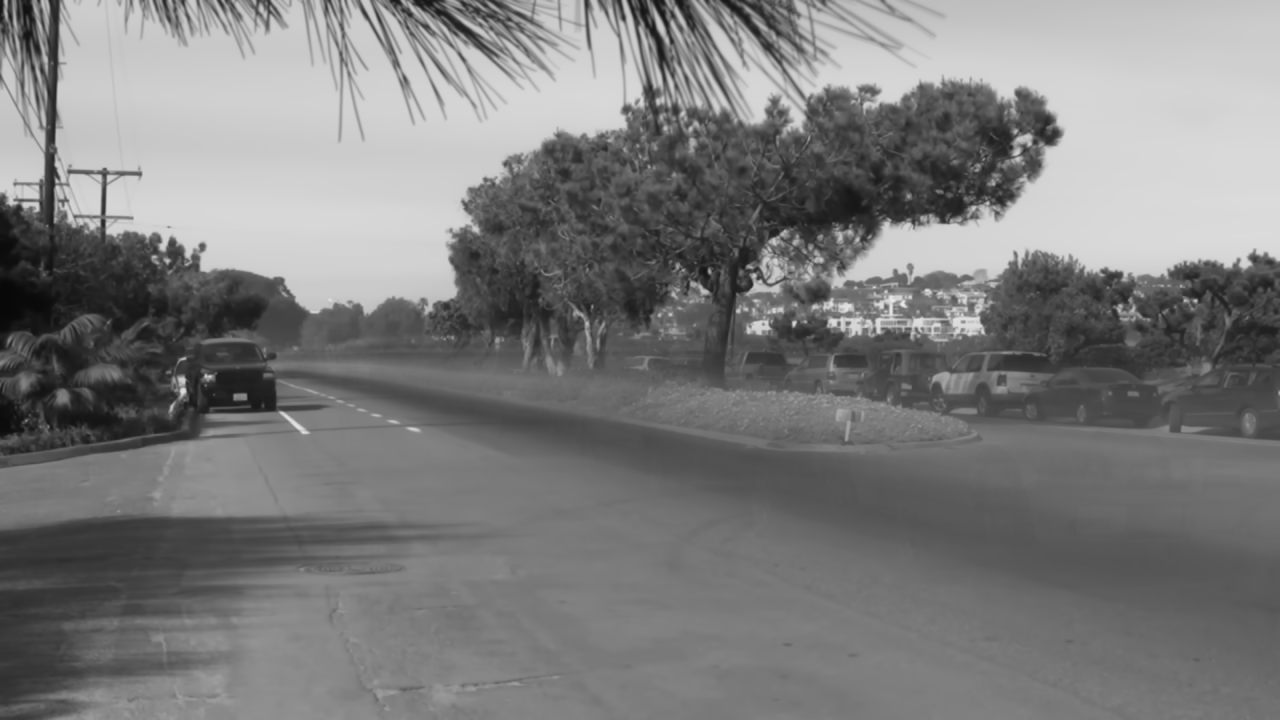
\includegraphics[width=0.7\linewidth]{_images/averageImage_spatiotemporalCars.png}
	\caption{Averages of the clouds and cars footage.}
	\label{fig:spatiotemporalsecondavg}
\end{figure}

The images look a lot better now. One thing that stood a bit out is when we look at the mountains. They almost look the same, that's because the clouds throw shade onto them which is actually not static anymore.


I had another idea to more reliably improve the above algorithm by combining RLOF with it. Herby we would make again two runs one to generat the dense of of the video then use that as a mask on top of the video to generate the spatiotemporal video result, we would remove the non moving parts of the images. The result would not contain most of the static structures. Most as the dense of algorithm can have outliers.

I would have implemented this but there is no more time to implement it.


\newpage
\section*{Discussion}\label{Discussion}
What you learnt about this assignment? \\
and how the method can be improved or extended? \\
What problems did you run into?\\
I've learned a lot actually. What RLOF is and the principle of it, I took a look at the paper of the Farneback optical flow algorithm. Also a bit more in depth about how we can improve sparse OF, when there aren't that many good edges in the scene, using another keypoint findung algorithm like SIFT.\\
An idea for implementing but less so for the assignment is in the exercise above.
\\
I've had a problem with the exercise to implement RLOF as I wanted to use the OpenCV optflow implementation, but there was always an error \\(\verb|cv2.error: OpenCV(4.7.0) /io/opencv_contrib/modules/ximgproc/src|\\\verb|/sparse_match_interpolators.cpp:204: error: (-215:Assertion failed)|\\\verb| match_num<SHRT_MAX in function 'interpolate'|).
And due to the fact that RLOF is almost not used, or at least the OpenCV implementation of it. There were no helpful resources online. I've tried to resolved the problem by trying a bit around, like changing the size of the window or changing the interpolator. But the real solution to the problem was to size the video down. In hindsight this makes sense. I've used a full HD video because that's the lowest resolution I can set on my phone. But that was seemingly a too high resolution. 


\end{document}
